% !TEX program = xelatex
\documentclass[fontset=windows, scheme=plain, 12pt, a4paper]{ctexart}

\usepackage[a4paper, top=2.5cm, bottom=2.5cm, left=2.5cm, right=2.5cm]{geometry}

\usepackage{amsmath}
\usepackage{url}
\usepackage{ragged2e}

\usepackage{multirow}
\usepackage{booktabs}
\usepackage{array}
\usepackage{graphicx}
\usepackage{float}
\usepackage{tabularx}   % Flexible-width tables and X columns.
\setlength{\intextsep}{5pt plus 1pt minus 1pt}
\setlength{\abovecaptionskip}{3pt}
\setlength{\belowcaptionskip}{3pt}
\graphicspath{{figures/}}
\IfFontExistsTF{Times New Roman}{\setmainfont{Times New Roman}}{}
\IfFontExistsTF{Consolas}{\setmonofont{Consolas}}{}

\linespread{1.6}
\setlength{\parindent}{2em}
\setlength{\emergencystretch}{2em}

\ctexset{
	section/number       = \arabic{section},
	subsection/number    = \arabic{section}.\arabic{subsection},
	subsubsection/number = \arabic{section}.\arabic{subsection}.\arabic{subsubsection},
}

\usepackage{titlesec}
\titleformat{\section}
{\centering\fontsize{14pt}{16.8pt}\bfseries}
{\arabic{section}.}{1em}{}
\titleformat{\subsection}
{\fontsize{12pt}{14.4pt}\bfseries}
{\arabic{section}.\arabic{subsection}}{1em}{}
\titleformat{\subsubsection}
{\fontsize{12pt}{14.4pt}\bfseries}
{\arabic{section}.\arabic{subsection}.\arabic{subsubsection}}{1em}{}
\titlespacing{\section}       {0pt}{1.0em}{-0.50em}
\titlespacing{\subsection}    {0pt}{1.18em}{-0.50em}
\titlespacing{\subsubsection} {0pt}{0.9em}{0.75em}

\usepackage{enumitem}
\usepackage{enumitem}
\setlist[enumerate]{
	label=\arabic*.,
    leftmargin=2.2em,     % Indentation of the whole list.
    labelsep=0.35em,      % Space between the number and the item text.
    itemsep=0em,          % Space between items.
    topsep=0.25em,        % Space above and below the list.
    parsep=0pt,           % Additional paragraph spacing within an item.
	partopsep=0pt
}

\usepackage{xcolor}
\usepackage{listings}
\lstset{
	basicstyle=\ttfamily\small,
	backgroundcolor=\color{black!3},
	frame=single,
	framesep=6pt,
	rulecolor=\color{black!30},
	framerule=0.8pt,
	breaklines=true,
	showstringspaces=false,
	columns=fullflexible,
	keepspaces=true,
}

\pagestyle{plain}

\newcommand{\referencescn}{%
	\begin{thebibliography}{99}
	\RaggedRight
	
	\setlength{\itemsep}{0pt}
	\setlength{\parskip}{0pt}
	\setlength{\parsep}{0pt}
	
	\linespread{1.5}\selectfont
	
	\setlength{\emergencystretch}{2em}
	
	\bibitem{ref1}
    Wang Jiye, Zhou Biyu, Zhang Fa, et al., [Review of Data Center Energy Consumption Models and Energy Efficiency Algorithms] (English translation of the Chinese title),
    Journal of Computer Research and Development, 56(8): 1587--1603, 2019.
	\bibitem{ref2}
    Ding Zhaohao, Cao Yujie, Zhang Sufang, et al., [Coordinated Optimization of Data Centers and Power Systems in the Energy Internet (I): Data Center Energy Consumption Models] (English translation of the Chinese title),
    Proceedings of the CSEE, 42(9): 3161--3176, 2022.
	\bibitem{ref3}
    L\"u Jiawei, Zhang Shenxi, Cheng Haozhong, et al., [Review and Prospects of Coordinated Energy-Flow and Data-Flow Planning for Integrated Energy Systems with Data Centers] (English translation of the Chinese title),
    Proceedings of the CSEE, 41(16): 5500--5521, 2021.
	
	\bibitem{ref4}
	Wickramasuriya S L, Athanasopoulos G, Hyndman R J,
	Optimal Forecast Reconciliation for Hierarchical and Grouped Time Series Through Trace Minimization,
	Journal of the American Statistical Association, 114(526): 804--819, 2019.
	
	\bibitem{ref5}
	Radovanovic A, Koningstein R, Schneider I, et al.,
	Carbon-Aware Computing for Datacenters,
	IEEE Transactions on Power Systems, 38(2): 1270--1280, 2023.
	
	\bibitem{ref6}
	Lindberg J, Lesieutre B C, Roald L A,
	Using Geographic Load Shifting to Reduce Carbon Emissions,
	Electric Power Systems Research, 212: 108586, 2022.
	
	\bibitem{ref7}
	Guo X, Che Y, Zheng Z, et al.,
	Multi-timescale Optimization Scheduling of Interconnected Data Centers Based on Model Predictive Control,
	Frontiers in Energy, 18(1): 28--41, 2024.
	
	\bibitem{ref8}
	Liu W, Yan Y, Sun Y, et al.,
	Online Job Scheduling Scheme for Low-carbon Data Center Operation: An Information and Energy Nexus Perspective,
	Applied Energy, 338: 120918, 2023.
	
	\bibitem{ref9}
    Xiang Ziyang, Huang Chunyi, Li Kangping, et al., [Coordinated Computing--Electricity Scheduling of Data Center Clusters Considering Spatial and Temporal Load Shifting] (English translation of the Chinese title),
    Electric Power Information and Communication Technology, 24(3): 33--46, 2026.
	
	\bibitem{ref10}
	Wang K, Ye L, Yang S, et al.,
	A Hierarchical Dispatch Strategy of Hybrid Energy Storage System in Internet Data Center with Model Predictive Control,
	Applied Energy, 331: 120414, 2023.

	\bibitem{ref11}
    DeepSeek, DeepSeek-v4-flash-0731, DeepSeek, used August 7--10, 2026.
	
\end{thebibliography}
%
}
\newcommand{\appendixcn}{%
    \section*{Appendix A\quad Core Code}%
	\section*{Appendix}

\subsection*{A. Software Environment and Reproduction}

Calculations use Python 3.12.13, with NumPy, pandas, Matplotlib, Seaborn, OpenPyXL, SciPy, and HiGHS for scientific computing, data processing, plotting, and optimization. The environment is managed by \texttt{uv}. Dependency constraints and locked versions are recorded in \texttt{pyproject.toml} and \texttt{uv.lock} in the supporting materials.

To reproduce results, first synchronize the environment, then execute the problem-level entry points in order from Problem 1 to Problem 4, working in the repository's \texttt{code/} directory. Preprocessing for Problems 2--4 depends on the shared processed layer generated by Problem 1. Run:

\begin{lstlisting}[language={},basicstyle=\ttfamily\small]
uv sync
uv run python question\question_01\main.py
uv run python question\question_02\main.py
uv run python question\question_03\main.py
uv run python question\question_04\main.py
\end{lstlisting}

Each entry point performs data processing, model solving, validation, and plotting in sequence. The supporting materials retain processed model inputs and generated result tables. To check published values, inspect result and independent-verification tables directly. To recompute from raw attachments, repeat preprocessing while preserving the original problem data.

\subsection*{B. Source Code and Supporting Materials}

Supporting materials include all source programs, environment configuration, processed model inputs, key result and validation tables for Problems 1--4, paper figures, and file checksum inventories. Result tables trace specific reported values; figures present results; independent-verification tables check job coverage, resource capacity, energy balance, storage states, and time boundaries.

Problem-specific evidence includes demand forecasting, baseline scheduling, and stress boundaries for Problem 1; multiobjective scheduling, baseline comparison, resource--energy recomputation, and sensitivity tests for Problem 2; storage optimization, regional metrics, baseline checks, and constraint tests for Problem 3; and joint computing--storage--electricity scheduling, scenarios, representative-window tests, and independent verification for Problem 4.

\subsection*{C. Limits on Result Interpretation}

Reported values come from the corresponding result tables, not estimates from figures. Passing hard-constraint checks establishes feasibility only for the given data, parameters, and boundaries. It does not establish global optimality or universal superiority across scenarios. Matheuristic results are reported with their actual solution method, comparison tests, and remaining limitations.

Hours 0--2399 form the main operating period; hours 2400--2405 complete already arrived jobs; hour 2406 is the terminal settlement boundary, not an ordinary execution hour. Costs including electricity sale revenue are net settlement values and do not imply negative actual electricity consumption.

\subsection*{D. AI Tool Use Details}

The team used DeepSeek during the competition for language editing, code debugging, figure preparation, and LaTeX typesetting assistance. AI was not used to determine core models, formulas, parameters, raw data, or final conclusions.

\subsubsection*{D.1 Tool and Dates of Use}

\begin{table}[H]
    \centering
    \small
    \renewcommand{\arraystretch}{1.05}
    \setlength{\tabcolsep}{3pt}
    \begin{tabularx}{0.96\textwidth}{>{\centering\arraybackslash}p{0.18\textwidth}>{\centering\arraybackslash}p{0.20\textwidth}>{\centering\arraybackslash}X>{\centering\arraybackslash}p{0.22\textwidth}}
        \toprule
        AI tool & Version/model & Developer & Dates of use \\
        \midrule
        DeepSeek & DeepSeek-v4-flash-0731 & DeepSeek & August 7--10, 2026 \\
        \bottomrule
    \end{tabularx}
\end{table}

The model version used was DeepSeek-v4-flash-0731.

\subsubsection*{D.2 Activities and Purposes}

DeepSeek assisted with language editing, debugging, figure preparation, final-draft compression, terminology consistency, citations, result-version checks, and LaTeX review. AI neither generated nor altered raw data and did not change the objectives, constraints, or parameters of the existing joint job search. Additional results were generated by actual local execution and independently recomputed.

\subsubsection*{D.3 Key Interaction Records}

\noindent\textbf{Record 1: DeepSeek language assistance, August 7--10, 2026}

The prompt requested review only of text written by the team, with local revision suggestions and no new models, formulas, data, or conclusions. AI identified long sentences, repetition, inconsistent terminology, and weak connections between text and figures. The team manually screened, checked, and rephrased suggestions.

\noindent\textbf{Record 2: Code debugging and figure assistance, August 9, 2026}

The prompt restricted review to syntax, indexing, data types, file reading, and plotting parameters in existing programs. It prohibited changes to raw data, objectives, constraints, model structure, parameters, and final conclusions. AI suggested variable checks, index corrections, data-type conversions, and figure-label improvements. The team adopted only suggestions reproducible locally without changing model meaning.

\noindent\textbf{Record 3: DeepSeek final-draft review, August 10, 2026}

The prompt required strict review of Problem 4 result accounting against a checklist, removal of mixed data versions across the sequential baseline, joint schedule, figures, and text, and consistent academic language, citations, and LaTeX formatting. AI assisted in adding entry points for consistent fixed-job energy recomputation and independent verification, and in revising plotting and paper sources. Every new metric was generated by actual execution on the team's computer; the team performed final checks and submission.

\subsubsection*{D.4 Adoption and Manual Revision}

The team checked all AI suggestions before adoption. Core methods, formulas, parameters, results, and conclusions were determined by the team, and final programs, data, figures, and conclusions were locally executed and verified. Complete DeepSeek records are contained in the corresponding use report in the supporting materials.

AI-assistance statements in the programs refer to the code checks and revisions involving DeepSeek. Assistance was limited to program review, result checking, figure preparation, and paper formatting; it did not rewrite the existing joint job-search model.

\subsection*{E. Source Inventory and Attachment Location}

All 24 Python source programs used for this problem were included in the source-code directory of the separately submitted support ZIP instead of being reprinted in the paper. That attachment also contains \texttt{pyproject.toml}, \texttt{uv.lock}, processed model inputs, key result and validation tables, paper figures, and a SHA-256 checksum inventory. Raw data supplied by the competition were not duplicated. The local readable copy is named \texttt{CCM2601033-support.zip}; the original competition package is retained in the frozen archive.

The source programs follow the relative directories for Problems 1--4 and comprise 24 \texttt{.py} files. Reproduction uses the commands in Appendix A in sequence. Paper and support attachments were submitted separately. The original attachment name followed the required problem-choice, entry-number, and attachment format, and its size was kept below 20 MB.
%
}
\newcommand{\threelinetable}[4]{%
	\begin{center}
		{\fontsize{10.5pt}{12.6pt}\bfseries #1}\par
		\vspace{-0.5em}
		\begin{tabular}{#2}
			\toprule
			#3 \\
			\midrule
			#4 \\
			\bottomrule
		\end{tabular}
	\end{center}
}

\renewcommand{\figurename}{Figure}
\renewcommand{\tablename}{Table}
\renewcommand{\refname}{References}
\begin{document}
	
	\begin{center}
		\renewcommand{\arraystretch}{1.25}
		\begin{tabularx}{\textwidth}{|>{\centering\arraybackslash}p{0.18\textwidth}|>{\centering\arraybackslash}X|>{\centering\arraybackslash}p{0.18\textwidth}|}
			\hline
            Category
            & \multirow{2}{=}{\centering\fontsize{14pt}{16.8pt}\bfseries 2026 Huashu Cup Undergraduate Mathematical Modeling Competition}
            & Entry Number \\
			\cline{1-1} \cline{3-3}
            Undergraduate
			& 
			& CM2601033 \\
			\hline
		\end{tabularx}
	\end{center}
	
	\vspace{-1.0em}
	
	\begin{center}
        {\fontsize{16pt}{19.2pt}\bfseries Hierarchical Forecasting and Multiobjective Scheduling for Coordinated Computing, Storage, and Electricity in Multiregional Data Centers
		}
	\end{center}
	
	\vspace{-0.85em}
	
	\begin{center}
        {\fontsize{14pt}{16.8pt}\bfseries Abstract}
	\end{center}
	
	\vspace{-0.5em}
	
    For computing--electricity coordination across six regional data centers, we develop a framework of \textbf{hierarchical forecasting and a neutral baseline, carbon-aware scheduling, storage coordination under specified loads, and joint computing--storage--electricity optimization}.
	
    Sparse, heterogeneous GPU demand is forecast using three levels of \textbf{local means}, with \textbf{marginal consistency} recovering 18 cross-classified demand series. With a \textbf{72\,h historical window}, validation and test WAPE are \textbf{0.7241 and 0.6519}, both below the 24\,h same-hour baseline;
    lexicographic scheduling achieves \textbf{100\% local execution} of 538 jobs, with \textbf{3\,h} of cumulative waiting.
	
    A \textbf{four-metric model} of net operating cost, carbon emissions, network latency, and renewable nonutilization is solved by a \textbf{rolling method with fixed normalization}. Relative to the neutral computing-only baseline,
    net operating cost decreases by \textbf{507.34 units of CNY\,10,000} and renewable utilization increases by \textbf{0.2232 percentage points},
    while carbon emissions and average network latency increase by \textbf{1.2752\,tCO$_2$ and 7.9468\,ms}, respectively.
	
    Under the specified AI and non-AI IT loads, storage and electricity purchases and sales are optimized subject to \textbf{energy conservation, SOC dynamics, and grid transaction limits}.
    Compared with a no-storage counterfactual, net operating cost decreases by \textbf{3936.19 units of CNY\,10,000},
    carbon emissions decrease from \textbf{8.8506\,tCO$_2$ to 0},
    and the sum of regional peak net grid purchases decreases from \textbf{31.5979\,MW to 0}.
	
    Joint optimization of job migration, start times, storage, and grid transactions yields a \textbf{six-metric model} of cost, emissions, latency, waiting loss, renewable nonutilization, and peak net grid purchases, solved using \textbf{fixed-normalization rolling optimization}. To remove degeneracy in the previous sequential energy solution, both sequential and joint job schedules are reevaluated under identical energy accounting. The joint job schedule reduces net operating settlement by \textbf{65.67 units of CNY\,10,000},
    lowers average network latency from \textbf{12.95\,ms to 9.96\,ms}, waiting loss by \textbf{0.004378}, and renewable nonutilization by \textbf{0.0258 percentage points};
    carbon emissions and peak net grid purchases increase by \textbf{41.08\,tCO$_2$ and 30.61\,MW}, revealing trade-offs between service quality, renewable utilization, and energy-side metrics.
	
    Scenario analysis shows that tighter carbon constraints reduce emissions by \textbf{30.53\%--100\%}; fixed regional average electricity prices increase net operating cost by \textbf{91.71 units of CNY\,10,000} and peak net grid purchases by \textbf{48.27\%}; complete smoothing within nonzero renewable-output periods reduces emissions by \textbf{88.12\%}.
	
    \textbf{Out-of-sample tests and independent full-horizon recomputation} confirm compliance with job, resource, energy, SOC, and grid transaction constraints. The \textbf{rolling matheuristic produces computationally efficient feasible schedules satisfying all hard constraints; global optimality is not claimed}.
    Joint decisions quantify trade-offs among cost, emissions, service quality, renewable utilization, and peak reduction.
	
    \noindent\textbf{Keywords:} computing--electricity coordination; hierarchical demand forecasting; carbon-aware scheduling; coordinated storage optimization; multiobjective optimization
	
	
	
	\newpage
	
	\section{Problem Restatement}

\subsection{Background}

The expansion of artificial intelligence increases both computing demand and energy consumption in data centers. Energy models must consider IT loads, facility efficiency, and electricity interactions\cite{ref1,ref2}; integrated energy systems must also coordinate data and energy flows\cite{ref3}. Regional differences in computing capacity, electricity prices, carbon intensity, renewable energy, and network latency, together with renewable fluctuations and job deadlines, create a multiregional, intertemporal computing--storage--electricity optimization problem.


\subsection{Problem Analysis}

\textbf{Problem 1:} Forecast GPU demand by region and job type for hours 2376--2399. Then use actual arriving jobs to select execution regions and start times under deadline, latency, GPU, and power constraints, establishing a baseline computing schedule.

\textbf{Problem 2:} Reschedule job regions and start times using actual jobs and energy parameters, developing a carbon-aware model balancing operating cost, emissions, network latency, and renewable utilization.

\textbf{Problem 3:} Fix the specified computing loads and optimize only renewable allocation, storage charging and discharging, and electricity purchases and sales. Evaluate storage effects on cost, emissions, peak net purchases, and fluctuations.

\textbf{Problem 4:} Jointly optimize job scheduling, storage, and grid transactions. Compare the joint schedule, the sequential baseline, and operating scenarios subject to computing, energy, and service-quality constraints.


\subsection{Overall Methodology}
As shown in Figure~\ref{fig:framework}, Problem 1 establishes a computing-only baseline; Problem 2 introduces prices, carbon intensity, and renewables; Problem 3 examines storage under fixed loads; and Problem 4 jointly releases job and energy decisions. This forms the progression from basic computing through computing--electricity coordination and storage regulation to joint computing--storage--electricity scheduling.


\begin{figure}[H]
	\centering
    \includegraphics[width=0.80\textwidth]{figures/workflow.pdf}
    \caption{Overall methodology for multiregional computing--storage--electricity coordination}
	\label{fig:framework}
\end{figure}

	% Problem analysis is included in Section 1.

	\section{Model Assumptions}

To use consistent modeling conventions across all problems, we make the following assumptions within the specified conditions:
\begin{enumerate}
    \item Once started, a job executes continuously and cannot be preempted, split, or migrated again during execution.
    \item Job start times are integer hours. Minute-resolution durations are converted to hourly GPU and power occupancy using the actual overlap with each hourly interval.
    \item AI IT power follows the specified common power mapping; non-AI IT loads are known hourly and cannot be migrated.
    \item Cross-region jobs incur only the specified network latency. Additional bandwidth limits, transferred data volumes, and transmission energy are excluded.
    \item Each region settles energy independently. Storage cannot charge and discharge simultaneously and must satisfy capacity, power, and terminal SOC constraints.
\end{enumerate}

	\section{Notation}

Table~\ref{tab:symbols} defines the main symbols.
Problem-specific parameters and auxiliary variables are defined in the corresponding models.

\begin{table}[H]
	\centering
    \caption{Main symbols and definitions}
	\label{tab:symbols}
	
	\small
	\renewcommand{\arraystretch}{0.85}
	
	\begin{tabularx}{0.96\textwidth}{
			>{\centering\arraybackslash}p{0.20\textwidth}
			>{\raggedright\arraybackslash}X
			>{\centering\arraybackslash}p{0.15\textwidth}}
		\toprule
        \textbf{Symbol} & \multicolumn{1}{c}{\textbf{Definition}} & \textbf{Unit} \\
		\midrule
		
		$i,r,t,s$
        & Indices of jobs, regions, periods, and candidate start times
		& -- \\
		
		$a_i,e_i,o_i,d_i$
        & Arrival time, earliest start, latest completion, and duration
		& h \\
		
		$g_i$
        & GPU demand of job $i$
		& GPU \\
		
		$p_i$
        & AI IT power of job $i$
		& MW \\
		
		$l_{ir},\,l_i^{\max}$
        & Execution latency and maximum permitted latency
		& ms \\
		
		$x_{irs}$
        & Whether job $i$ starts in region $r$ at time $s$
		& $\{0,1\}$ \\
		
		$\rho_{ist}$
        & Fraction of period $t$ occupied by job $i$
		& -- \\
		
		$P^{AI}_{rt},\,P^{NonAI}_{rt}$
        & AI and non-AI IT loads
		& MW \\
		
		$F_{rt}$
        & Total facility load in region $r$
		& MW \\
		
		$G^{ava}_{rt}$
        & Available GPU capacity in region $r$
		& GPU \\
		
		$PUE_r$
        & PUE of region $r$
		& -- \\
		
		$P^{RE}_{rt}$
        & Available renewable power in region $r$
		& MW \\
		
		$\pi_{rt},\,\sigma_{rt}$
        & Electricity purchase and sale prices
        & CNY/MWh \\
		
		$\kappa_{rt}$
        & Grid carbon intensity
		& tCO$_2$/MWh \\
		
		$B_{rt},\,X_{rt},\,R_{rt}$
        & Grid purchase, renewable export, and curtailed power
		& MW \\
		
		$S_{rt}$
        & Stored energy at the start of period $t$
		& MWh \\
		
		\bottomrule
	\end{tabularx}
\end{table}

	\section{Model Formulation and Solution for Problem 1}

\subsection{Data Preprocessing}

The raw data contain 50000 jobs, 6 regions, and 3 job types, with arrivals spanning hours 0--2399. After checking field completeness and value ranges, durations are converted from minutes to hours, per-GPU power is matched by job type, and candidate regions are screened by maximum network latency. Physical quantities are neither standardized nor filtered for outliers. Forecasting data are aggregated by arrival hour, source region, and job type, including zero-demand combinations, yielding 43200 records. Hours 0--2351, 2352--2375, and 2376--2399 form the training, validation, and test sets, respectively. Scheduling uses actual test-period jobs directly; hours 2400--2405 allow unfinished execution, and hour 2406 is the terminal boundary.


\subsection{Model Formulation}

Problem 1 treats short-term GPU forecasting and baseline computing scheduling separately. Forecasts are used only for accuracy evaluation and do not enter actual scheduling.

Let $D_{rkt}$ denote newly arriving GPU demand in region $r$ for job type $k$ at time $t$,
and let $g_i$ denote the GPU demand of job $i$. Then
\begin{equation}
	D_{rkt}
	=
	\sum_{\substack{i:\,a_i=t\\
			r_i^0=r,\;k(i)=k}}
	g_i .
	\label{eq:q1_demand}
\end{equation}

This produces 18 bottom-level series, together with regional demand $D_{rt}=\sum_kD_{rkt}$, job-type demand $D_{kt}=\sum_rD_{rkt}$, and system demand $D_t=\sum_rD_{rt}$. Bottom-level series retain heterogeneity, while the three aggregate levels improve short-term forecasting stability.

Hierarchical and grouped time series require forecast reconciliation for cross-level consistency\cite{ref4}. We construct a nonnegative prior from historical demand shares and use generalized KL divergence to recover 18 cross-classified demands. This follows the reconciliation principle without directly using the Trace MinT objective.

For an aggregate demand series $y_t$,
the mean of the most recent $H$ historical hours predicts the next 24 hours:
\begin{equation}
	\hat{y}_{T+h}(H)
	=
	\frac{1}{H}
	\sum_{\tau=T-H+1}^{T}y_{\tau},
	\qquad h=1,2,\ldots,24 .
	\label{eq:q1_localmean}
\end{equation}

Here $T$ is the last observed time before forecasting. The validation set selects a window from $H\in\{24,72,168,336\}$; hours 0--2375 then forecast hours 2376--2399. Test observations do not enter model selection.

Separate regional, job-type, and system forecasts may have inconsistent totals.
We therefore use the system forecast $\hat D_t^{(S)}$ as the total-demand anchor,
proportionally rescale the regional and job-type marginals,
and obtain $\tilde D_{rt}$ and $\tilde D_{kt}$.
Let $q_{rk}$ denote the historical mean regional--job-type demand share.
A prior with the same units as GPU demand is defined as
$q^0_{rkt}=q_{rk}\hat D_t^{(S)}$;
Zero historical shares are assigned a small positive value to avoid logarithmic singularities.
Generalized KL divergence then recovers the 18 cross-classified demands:
\begin{equation}
	\begin{aligned}
		\min_{z_{rkt}\geq0}\quad
		&\sum_r\sum_k
		\left[
		z_{rkt}\ln\frac{z_{rkt}}{q^0_{rkt}}
		-z_{rkt}+q^0_{rkt}
		\right],\\
		\mathrm{s.t.}\quad
		&\sum_kz_{rkt}=\tilde D_{rt},\\
		&\sum_rz_{rkt}=\tilde D_{kt}.
	\end{aligned}
	\label{eq:q1_kl}
\end{equation}

Equation~(\ref{eq:q1_kl}) keeps the two sets of marginals fixed while retaining the historical structure of the 18 demands. WAPE, RMSE, and MAE evaluate forecasts against demand at the same hour 24 hours earlier.

Baseline computing scheduling uses actual jobs arriving during hours 2376--2399.
Let job $i$ have duration $d_i$ and source region $r_i^0$.
Network latency determines candidate regions $R_i$.
Real-time inference jobs start immediately on arrival;
batch inference and AI training jobs have candidate start times $S_i$ consistent with earliest start, latest completion, and the terminal boundary at 2406.
The binary variable $x_{irs}$ indicates whether job $i$ starts in region $r$ at time $s$.

Job durations retain minute precision, while resource capacities are evaluated hourly.
The actual occupancy of interval $[t,t+1)$ for job $i$ starting at $s$ is
\begin{equation}
	\rho_{ist}
	=
	\max\left\{
	0,\,
	\min(s+d_i,t+1)-\max(s,t)
	\right\}.
	\label{eq:q1_overlap}
\end{equation}

Equation~(\ref{eq:q1_overlap}) gives hourly GPU and power occupancy.
The AI IT power of job $i$ during full execution is
$p_i=g_iP^{GPU}_{k(i)}$.
The effective IT power available to AI jobs in region $r$ at time $t$ is
\[
A_{rt}
=
\max\left\{
0,\,
\min\left(
P^{IT,\max}_r-P^{NonAI}_{rt},
\frac{P^{Facility,\max}_r}{PUE_r}-P^{NonAI}_{rt}
\right)
\right\}.
\]
The main resource constraints are
\begin{equation}
	\begin{aligned}
		&\sum_{r\in R_i}\sum_{s\in S_i}x_{irs}=1,
		&&\forall i,\\
		&\sum_i\sum_{s\in S_i}
		g_i\rho_{ist}x_{irs}
		\leq G^{ava}_{rt},
		&&\forall r,t,\\
		&\sum_i\sum_{s\in S_i}
		p_i\rho_{ist}x_{irs}
		\leq A_{rt},
		&&\forall r,t .
	\end{aligned}
	\label{eq:q1_capacity}
\end{equation}

Equation~(\ref{eq:q1_capacity}) ensures unique execution and feasible GPU and power occupancy. Candidate sets $R_i$ and $S_i$ exclude combinations violating latency, time windows, or the terminal boundary.

Problem 1 excludes prices, emissions, renewables, and storage,
providing a neutral computing baseline for subsequent computing--electricity coordination.
First minimize cross-region migrated GPU work,
then minimize cumulative waiting of flexible jobs conditional on the optimal first-level objective:
\begin{equation}
	\begin{aligned}
		\min\quad
		F_1
		&=
		\sum_i
		\sum_{\substack{r\in R_i\\r\neq r_i^0}}
		\sum_{s\in S_i}
		g_id_ix_{irs},\\
        \text{subject to }F_1=F_1^{*}\text{,}\qquad
		\min\quad
		F_2
		&=
		\sum_{i\in I^{\mathrm{flex}}}
		\sum_{r\in R_i}\sum_{s\in S_i}
		(s-e_i)x_{irs}.
	\end{aligned}
	\label{eq:q1_objective}
\end{equation}

Here $F_1$ measures migrated GPU work and $F_2$ measures cumulative waiting of flexible jobs.


\subsection{Results and Model Validation}

The validation set gives the lowest overall WAPE at $H=72$. Historical data from hours 0--2375 therefore forecast the 18 GPU-demand series for hours 2376--2399.

The cumulative AI-training GPU demands in RegionD, RegionE, and RegionF are
407683, 292000, and 296143, respectively,
substantially above the corresponding values in RegionA, RegionB, and RegionC:
63070, 62551, and 58899.
Bottom-level hourly demand also contains many low values and random spikes,
making direct forecasts of the 18 fine-grained series sensitive to random job arrivals.

\begin{table}[H]
	\centering
    \caption{Forecast errors of the hierarchical model and the 24-hour same-hour baseline}
	\label{tab:q1_forecast}
	
	\fontsize{10.5pt}{12pt}\selectfont
	\renewcommand{\arraystretch}{0.88}
	
	\begin{tabular}{ccccccc}
		\toprule
        \multirow{2}{*}{\textbf{Period}}
        & \multicolumn{3}{c}{\textbf{Hierarchical local mean}}
        & \multicolumn{3}{c}{\textbf{24-hour same-hour baseline}}\\
		\cmidrule(lr){2-4}\cmidrule(lr){5-7}
		& \textbf{WAPE} & \textbf{RMSE} & \textbf{MAE}
		& \textbf{WAPE} & \textbf{RMSE} & \textbf{MAE}\\
		\midrule
        Validation
		& 0.7241 & 45.7417 & 23.6915
		& 1.0957 & 69.9249 & 35.8495\\
		
        Test
		& 0.6519 & 53.4704 & 26.3323
		& 0.8740 & 72.8628 & 35.3032\\
		\bottomrule
	\end{tabular}
\end{table}


Table~\ref{tab:q1_forecast} shows that all three errors of the hierarchical model are below the baseline in both validation and test periods. The problem separately requires short-term forecasting and final-period computing scheduling; forecasts assess demand predictability, while actual jobs arriving during hours 2376--2399 remain the scheduling input so that forecasting errors cannot alter job-level feasibility. Validation and test WAPE of 0.7241 and 0.6519 show that sparse demand and random spikes remain difficult to predict. Lower test WAPE and higher RMSE are consistent: WAPE is normalized by total observed demand, whereas RMSE is more sensitive to a few large errors.

\begin{figure}[H]
	\centering
	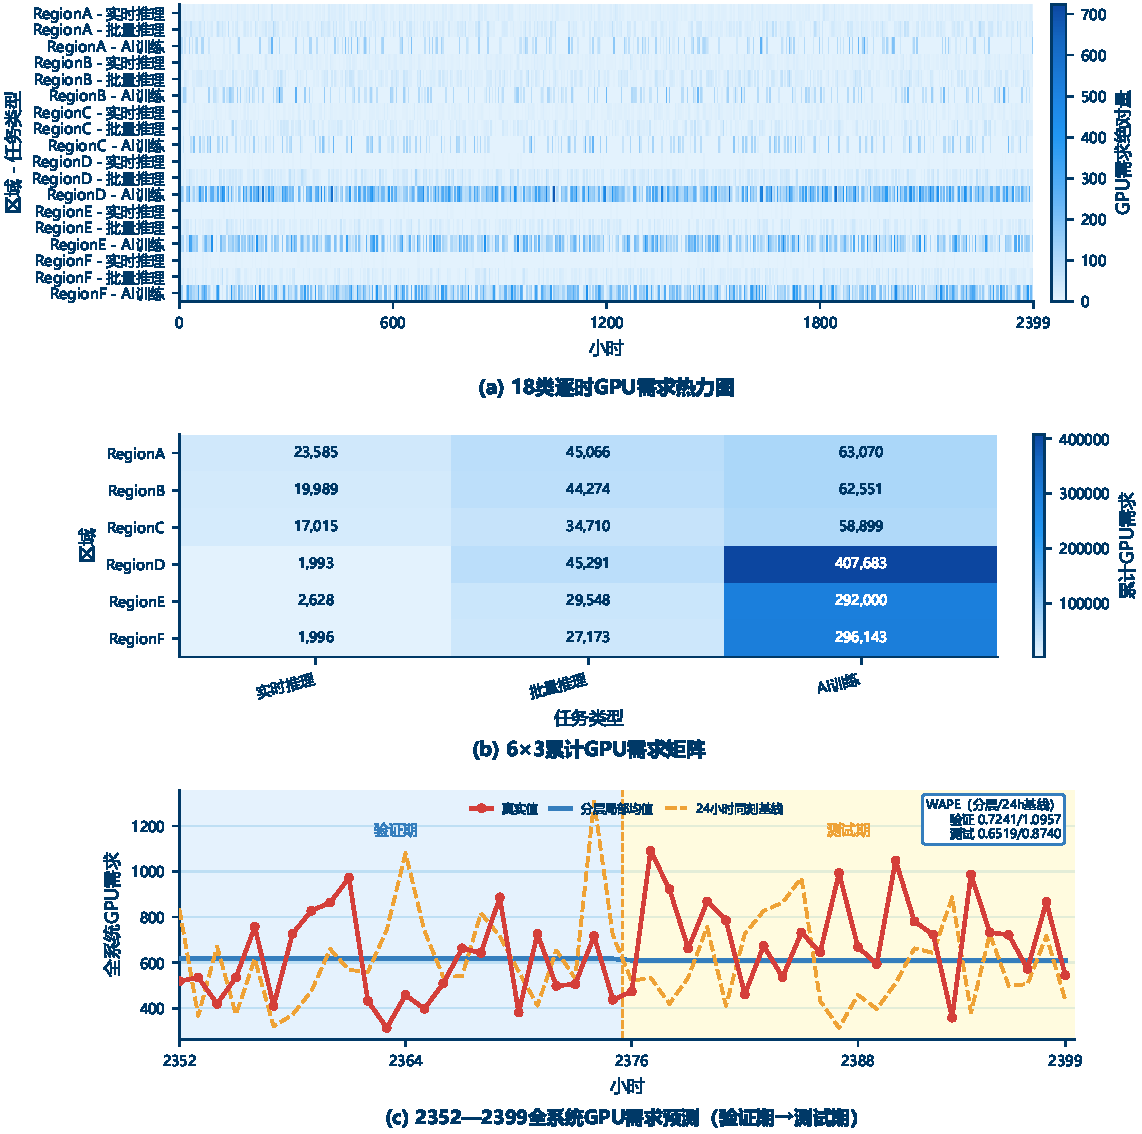
\includegraphics[width=0.80\textwidth]{figures/q1_group1_demand_structure.pdf}
    \caption{GPU-demand heterogeneity and hierarchical short-term forecasts}
	\label{fig:q1_forecast}
\end{figure}

Figure~\ref{fig:q1_forecast} shows that the model captures short-term demand levels rather than random single-hour spikes.

The 538 actual jobs arriving during hours 2376--2399 undergo two-level optimization using Equation~(\ref{eq:q1_objective}).

\begin{table}[H]
	\centering
    \caption{Baseline computing scheduling results}
	\label{tab:q1_dispatch}
	
	\fontsize{10.5pt}{12pt}\selectfont
	\renewcommand{\arraystretch}{0.88}
	
	\begin{tabular}{cc}
		\toprule
        \textbf{Metric} & \textbf{Result}\\
		\midrule
        Number of jobs & 538\\
        First-level objective $F_1^*$ & $0$ GPU$\cdot$h\\
        Local execution rate & 100\%\\
        Second-level objective $F_2^*$ & 3 h\\
        Relative optimality gap & 0\\
		\bottomrule
	\end{tabular}
\end{table}


In Table~\ref{tab:q1_dispatch}, $F_1^*=0$ and $F_2^*=3$ h. All 538 jobs finish in their source regions; the current resources permit feasible execution without migration.

\begin{figure}[H]
	\centering
	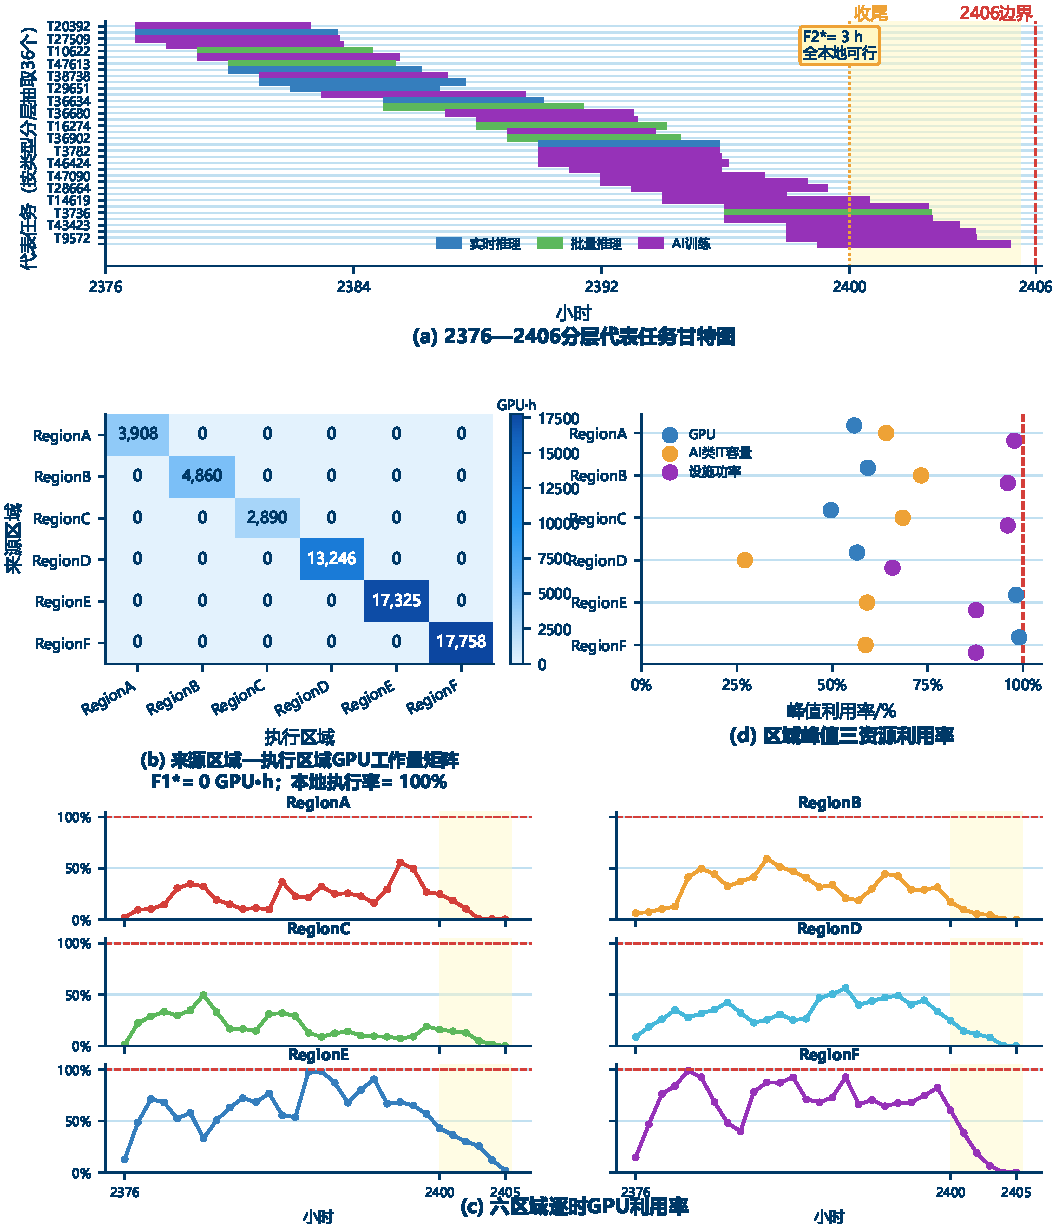
\includegraphics[width=0.75\textwidth]{figures/q1_group2_core_results.pdf}
    \caption{Baseline computing schedule and multiple-resource occupancy}
	\label{fig:q1_dispatch}
\end{figure}

Figure~\ref{fig:q1_dispatch} shows completion of all final-period jobs before 2406 and a regional GPU-work matrix with nonzero entries only on its main diagonal. RegionE and RegionF approach GPU limits during some hours, while certain eastern regions are constrained by facility power.

The hierarchical model has lower WAPE than the 24-hour same-hour baseline in all 84 rolling out-of-sample windows; a one-sided Wilcoxon test gives $p=8.55\times10^{-16}$.

The median WAPE difference between reconciled and direct forecasts is $-3.05\times10^{-4}$ ($p=0.216$). Maximum regional and job-type marginal closure errors are both $6.82\times10^{-13}$, and the 18-class aggregate error is $4.11\times10^{-10}$. Reconciliation ensures cross-level closure rather than improving accuracy.

\begin{figure}[H]
	\centering
	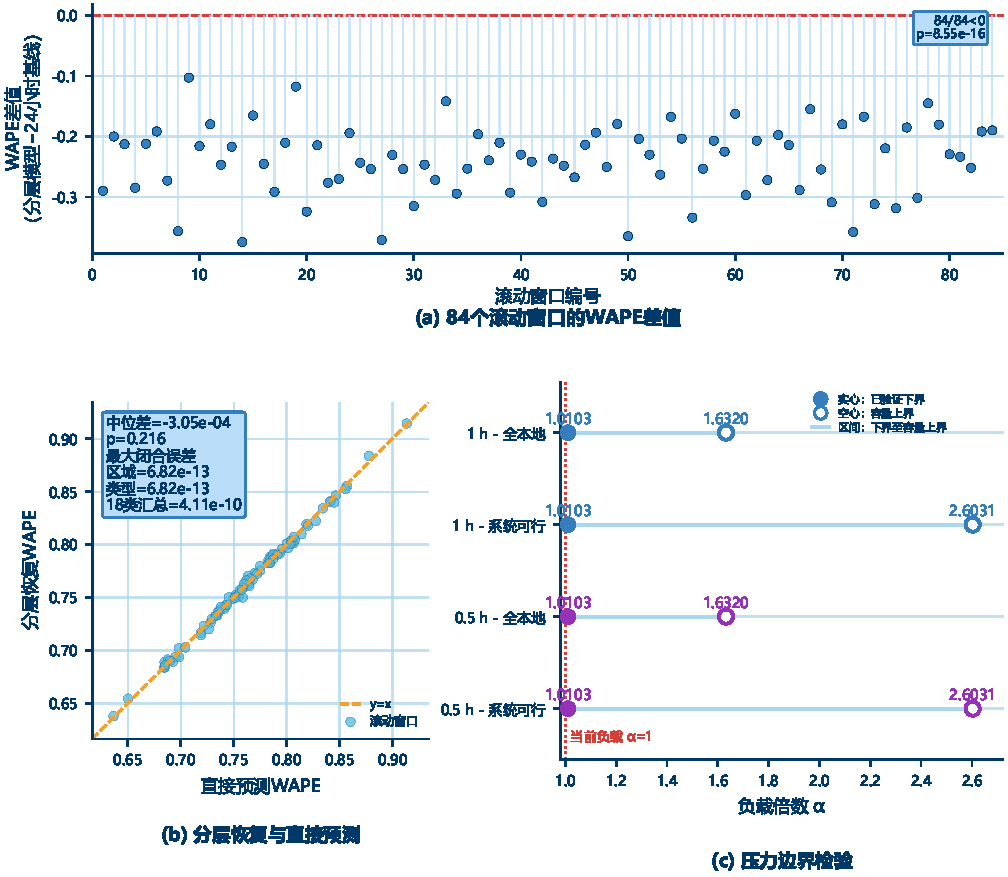
\includegraphics[width=0.80\textwidth]{figures/q1_group3_validation_robustness.pdf}
    \caption{Forecast stability and computing-schedule stress boundaries}
	\label{fig:q1_validation}
\end{figure}

In Figure~\ref{fig:q1_validation}, the verified feasible lower bound on load multiplier $\alpha$ is 1.0103. The theoretical capacity upper bounds for fully local execution and cross-region coordination are 1.6320 and 2.6031; these latter values are not verified exact critical thresholds.

Recomputation with 0.5-hour granularity still yields $F_1^*=0$, while cumulative waiting falls from 3 h to 2 h. The conclusion that migration is unnecessary remains unchanged. Unique execution, immediate real-time starts, latency, deadlines, and all capacity constraints show no violations.

Problem 1 thus establishes short-term demand forecasts and a computing-only baseline for comparison after Problem 2 introduces energy factors.

	\section{Model Formulation and Solution for Problem 2}

\subsection{Model Formulation}

Problem 2 reoptimizes execution regions and start times using actual jobs and hourly electricity parameters for hours 0--2399; forecasts do not enter scheduling. Hours 2400--2405 are reserved for completion and settlement, and all jobs must finish before 2406. Storage is excluded.
Research on carbon-aware data centers identifies grid carbon intensity as an important signal for job scheduling and energy management\cite{ref5}.
Cross-region load shifting exploits regional differences in electricity and carbon conditions,
but introduces network latency and service-quality costs\cite{ref6}.
Accordingly, we evaluate cost, emissions, communication latency, and renewable utilization subject to deadlines, latency, GPU, and power constraints.

Job parameters and fractional hourly occupancy follow Problem 1. Real-time jobs start immediately, while flexible jobs may shift within their valid time windows.
Let $x_{irs}$ indicate whether job $i$ starts in region $r$ at time $s$.
Candidate regions $R_i$ satisfy network latency limits,
and candidate start times $S_i$ satisfy arrival, completion, and terminal constraints at 2406.

The AI IT load, total IT load, and facility load in region $r$ at time $t$ are denoted by
$P^{AI}_{rt}$, $P^{IT}_{rt}$, and $F_{rt}$, respectively.
Using fractional occupancy from Equation~(\ref{eq:q1_overlap}),
\begin{equation}
	\begin{aligned}
		P^{AI}_{rt}
		&=
		\sum_i\sum_{s\in S_i}
		p_i\rho_{ist}x_{irs},\\
		P^{IT}_{rt}
		&=
		P^{NonAI}_{rt}+P^{AI}_{rt},\\
		F_{rt}
		&=
		PUE_rP^{IT}_{rt}.
	\end{aligned}
	\label{eq:q2_load_mapping}
\end{equation}

Hourly GPU occupancy retains the Problem 1 constraints. IT capacity, facility capacity, and maximum grid purchase capacity define an effective AI IT limit
$\bar P^{AI}_{rt}
=\min\{P^{IT,\max}_{rt}-P^{NonAI}_{rt},
P^{Facility,\max}_{rt}/PUE_r-P^{NonAI}_{rt},
(P^{RE}_{rt}+P_r^{Grid,\max})/PUE_r-P^{NonAI}_{rt}\}$,
with $P^{AI}_{rt}\leq\bar P^{AI}_{rt}$; GPU, latency, and deadline constraints otherwise follow Problem 1.

Without storage, renewables first serve local loads. Grid purchases cover any deficit, exports use available surplus up to the export limit, and the remainder is curtailed.
Let $V_{rt}$, $B_{rt}$, $X_{rt}$, and $R_{rt}$ denote
direct renewable use, grid purchases, renewable exports, and curtailment, respectively. Then
\begin{equation}
	\begin{aligned}
		V_{rt}&=\min(F_{rt},P^{RE}_{rt}),\\
		B_{rt}&=\max(F_{rt}-P^{RE}_{rt},0),\\
		X_{rt}&=\min\{\max(P^{RE}_{rt}-F_{rt},0),\bar X_r\},\\
		R_{rt}&=P^{RE}_{rt}-V_{rt}-X_{rt},
	\end{aligned}
	\label{eq:q2_energy}
\end{equation}
Here $0\leq B_{rt}\leq P_r^{Grid,\max}$ and $0\leq X_{rt}\leq\bar X_r$.

The schedule is evaluated using net operating cost $C$, carbon emissions $E$, average network latency $L$,
and renewable utilization $U$.
For $t=0,\ldots,2405$, define
\begin{equation}
	\begin{aligned}
		C
		&=
		\sum_r\sum_{t=0}^{2405}
		\left(\pi_{rt}B_{rt}-\sigma_{rt}X_{rt}\right),\\
		E
		&=
		\sum_r\sum_{t=0}^{2405}\kappa_{rt}B_{rt},\\
		L
		&=
		\frac{1}{N}
		\sum_i\sum_{r\in R_i}\sum_{s\in S_i}
		l_{ir}x_{irs},\\
		U
		&=
		\frac{\displaystyle
			\sum_r\sum_{t=0}^{2405}(V_{rt}+X_{rt})}
		{\displaystyle
			\sum_r\sum_{t=0}^{2405}P^{RE}_{rt}},
		\qquad Q=1-U.
	\end{aligned}
	\label{eq:q2_objectives}
\end{equation}

Let $f_1=C,f_2=E,f_3=L,f_4=Q$. Single-objective continuous relaxations yield ideal lower bounds $f_m^{LB}$. Together with the computing-only baseline $f_m^0$ and single-objective anchors $x^{(a)}$, these define fixed normalization scales:
\begin{equation}
	\begin{aligned}
		f_m^{ref}
		&=
		\max\left\{
		f_m^0,\max_a f_m(x^{(a)})
		\right\},\\
		R_m
		&=
		f_m^{ref}-f_m^{LB},\\
		d_m(x)
		&=
		\frac{f_m(x)-f_m^{LB}}{R_m},\\
		\min\quad z,
		&\qquad d_m(x)\leq z,\quad \forall m .
	\end{aligned}
	\label{eq:q2_minmax}
\end{equation}

If $R_m\approx0$, the metric is used only for evaluation; otherwise Equation~(\ref{eq:q2_minmax}) minimizes the maximum normalized deviation.

Multiscale rolling optimization handles dynamic coupling among job arrivals, loads, and energy states\cite{ref7}; low-carbon online scheduling must also coordinate service quality and energy metrics\cite{ref8}. For 50000 jobs, we use a decision window of $H=24$ h and a look-ahead window of $K=48$ h, with feasibility repair and local mixed-integer linear programming refinement.
At rolling origin $\tau$,
we examine $[\tau,\tau+H+K)$,
but commit only jobs actually starting within $[\tau,\tau+H)$.
Already started jobs retain their existing schedules;
flexible jobs whose latest valid start enters the current window must start in this iteration.

The construction phase schedules real-time jobs first, then sorts flexible jobs by time slack and resource demand.
Define the current full-horizon objective estimate as
$\hat f_{m,\tau}
=f_m^0+\Delta f_{m,\tau}^{past}
+f_{m,\tau}^{scope}-f_{m,\tau}^{0,scope}$.
For each valid candidate $(r,s)$, compute
\begin{equation}
	S_{irs}
	=
	\max_m
	\left\{
	\frac{
		\hat f_{m,\tau}
		+\Delta f_{m,irs}
		-f_m^{LB}}
	{R_m}
	\right\},
	\qquad
	(r_i^*,s_i^*)
	=
	\arg\min_{(r,s)}S_{irs}.
	\label{eq:q2_marginal}
\end{equation}

Capacity conflicts trigger rescheduling of replaceable jobs. Once feasible, key jobs form a large neighborhood, and refinement fixes decisions outside that neighborhood. Table~\ref{tab:q2_algorithm} summarizes the procedure.

\begin{table}[H]
	\centering
    \caption{Rolling matheuristic for Problem 2}
	\label{tab:q2_algorithm}

	\fontsize{10.5pt}{12pt}\selectfont
	\renewcommand{\arraystretch}{0.88}

	\begin{tabular}{
			>{\centering\arraybackslash}p{0.08\textwidth}
			>{\raggedright\arraybackslash}p{0.86\textwidth}}
		\toprule
        \textbf{Step} & \multicolumn{1}{c}{\textbf{Operation}}\\
		\midrule

		1 &
        Determine fixed normalization scales from continuous relaxations, the Problem 2 computing-only baseline, and single-objective anchors.\\

		2 &
        Read the $H=24$ h decision window and $K=48$ h look-ahead interval;
        lock already started jobs and identify jobs required to start now.\\

		3 &
        Schedule real-time jobs immediately; sort flexible jobs by slack and resource demand,
        then use Equation~(\ref{eq:q2_marginal}) to select feasible candidates.\\

		4 &
        Update GPU occupancy, AI IT loads, and energy states;
        reschedule replaceable jobs when capacity conflicts occur.\\

		5 &
        Select key jobs to form a large neighborhood,
        fix decisions outside it, and refine using a small mixed-integer linear program.\\

		6 &
        Commit the current $H$-hour decisions and continue rolling;
        finally reconstruct the full profile for hours 0--2405 and verify it independently.\\

		\bottomrule
	\end{tabular}
\end{table}


Candidates are evaluated by the original multiobjective criterion; the matheuristic only restricts the integer search space. It produces computationally efficient feasible schedules satisfying all hard constraints; global optimality is not claimed.


\subsection{Results and Model Validation}

A full-horizon computing-only baseline for 50000 jobs follows the Problem 1 principles and is settled under Problem 2 energy accounting. Table~\ref{tab:q2_result} gives rolling optimization results.

\begin{table}[H]
	\centering
    \caption{Problem 2 multiobjective schedule versus its computing-only baseline}
	\label{tab:q2_result}

	\fontsize{10.5pt}{12pt}\selectfont
	\renewcommand{\arraystretch}{0.90}

	\begin{tabular}{lccc}
		\toprule
        \multicolumn{1}{c}{\textbf{Metric}}
        & \textbf{Computing baseline}
        & \textbf{Balanced schedule}
        & \textbf{Change}\\
		\midrule

        Net cost/CNY
		& $-4.196834\times10^8$
		& $-4.247568\times10^8$
        & $-507.34$ (CNY $10^4$)\\

        Emissions/tCO$_2$
		& 8.850562
		& 10.125791
        & $+1.275228$\\

        Mean latency/ms
		& 5.000000
		& 12.946840
        & $+7.946840$\\

        Renewable utilization
		& 67.91598\%
		& 68.13914\%
        & $+0.22316$ pp\\

        Mean waiting/h
		& 0.00116
		& 30.89284
        & $+30.89168$\\

        Migration share
		& 0
		& 29.35800\%
        & $+29.35800$ pp\\

		\bottomrule
	\end{tabular}
\end{table}


Table~\ref{tab:q2_result} shows a net cost reduction of 507.34 units of CNY $10^4$ and a renewable utilization increase of 0.22316 percentage points, alongside emission and mean latency increases of 1.2752 tCO$_2$ and 7.95 ms. Negative cost means export revenue exceeds electricity purchase expenditure.

With fixed normalization, the four deviations are 1.00, 1.00, 0, and 1.00 for the computing baseline, versus 0.85, 1.14, 1.15, and 0.87 for the Problem 2 schedule, giving a maximum deviation $z=1.15$.

\begin{figure}[H]
	\centering
	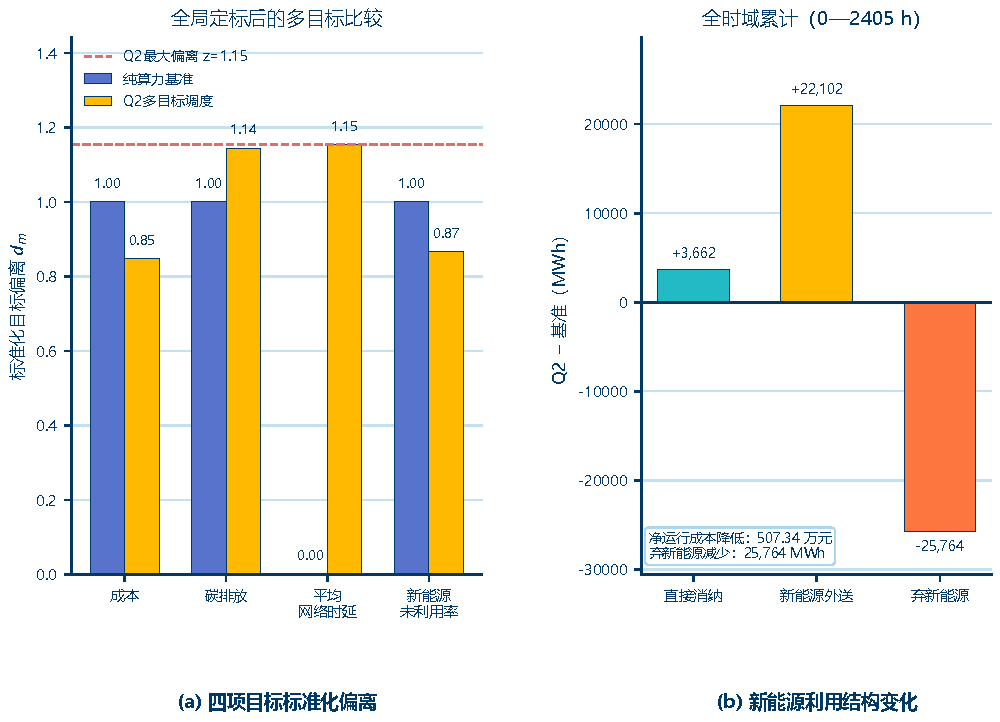
\includegraphics[width=0.82\textwidth]
	{figures/q2_group1_core_results.pdf}
    \caption{Problem 2 multiobjective results and changes in renewable utilization}
	\label{fig:q2_core}
\end{figure}

In Figure~\ref{fig:q2_core}, direct renewable use and exports increase by approximately 3662 and 22102 MWh, respectively, while curtailment falls by about 25764 MWh. These changes approximately balance.

Of all jobs, 35321 execute locally and 14679 migrate across regions. The migration share is 29.358\%, with migrated work of $1.308142\times10^6\,\mathrm{GPU\cdot h}$.

Figure~\ref{fig:q2_migration} shows more outward migration from D, E, and F, with C and D absorbing more cross-region computing work. Both resource and energy conditions influence migration directions.

Reconstructed profiles for hours 0--2405 from all 50000 job records preserve cumulative quantities in both schedules: AI IT energy is $7.389279853\times10^5$ MWh and GPU work is $5.020787\times10^6$ GPU$\cdot$h.
There are no job, latency, deadline, capacity, or grid purchase violations. Energy balance residuals are zero, and no job occupies resources at 2406.

Of 91 refinement windows, 45 accept improvements, with a mean improvement of 2.43\%. Exact comparisons for windows 0--9 give a median speedup of approximately 31.8, a mean absolute relative deviation of 39.82\%, and a maximum normalized-objective deviation of 293.40\%. The maximum is a relative deviation of the local-window normalized objective, not a full-horizon error in cost or emissions. However, it shows that restricted neighborhoods can miss better job combinations in some resource-constrained windows. We therefore describe the method only as a large-scale approximation satisfying all hard constraints, without claiming local or full-horizon optimality.

\begin{figure}[H]
	\centering
	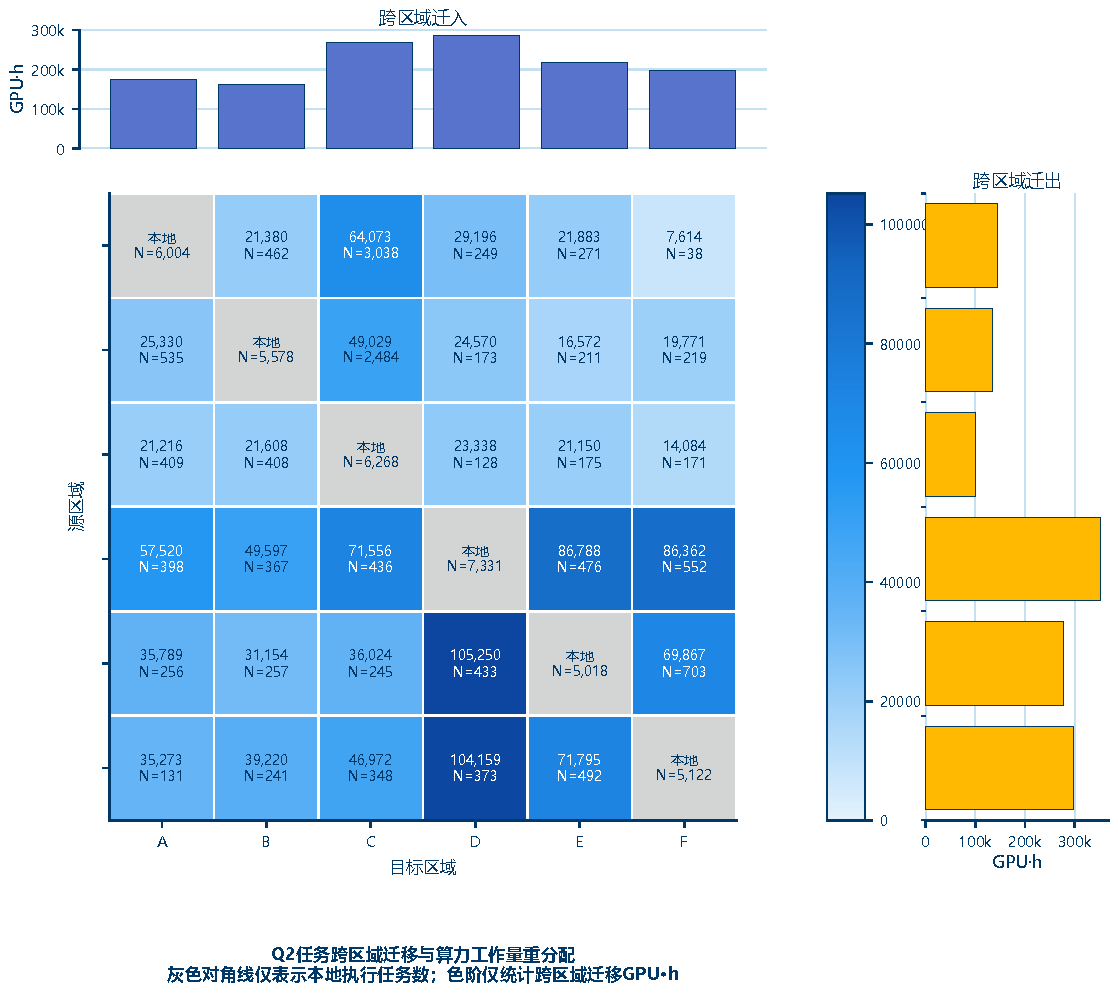
\includegraphics[width=0.68\textwidth]
	{figures/q2_group2_dispatch_mechanism.pdf}
    \caption{Cross-region job migration and computing-work redistribution in Problem 2}
	\label{fig:q2_migration}
\end{figure}

\begin{figure}[H]
	\centering
	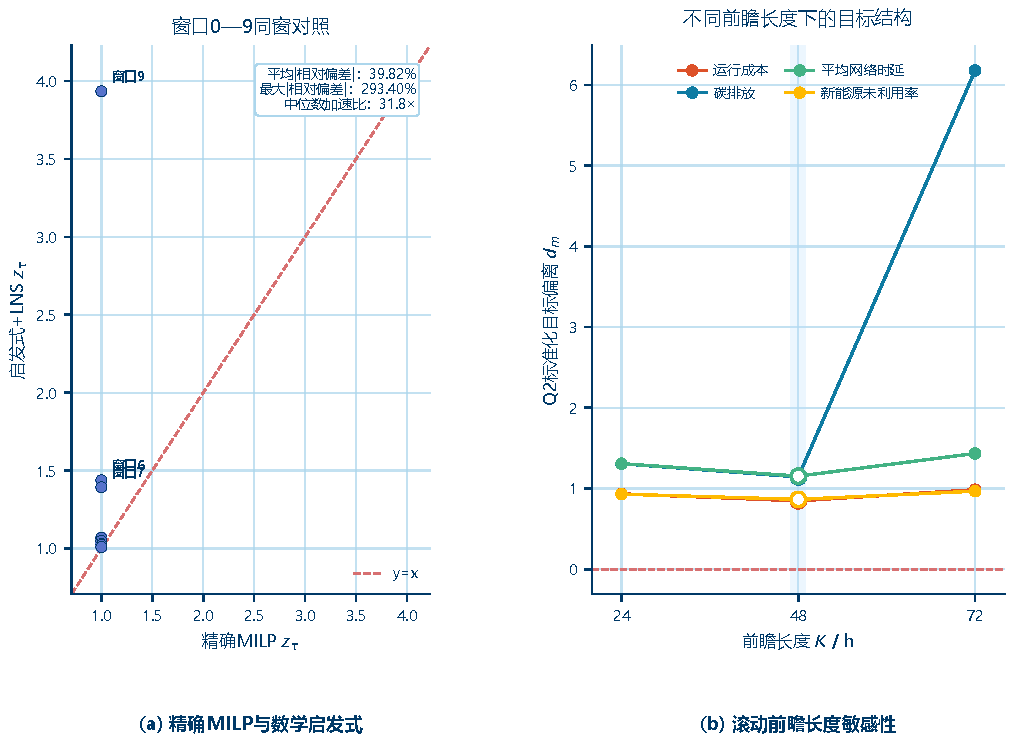
\includegraphics[width=0.72\textwidth]
	{figures/q2_group3_model_validation.pdf}
    \caption{Problem 2 matheuristic quality and look-ahead sensitivity}
	\label{fig:q2_validation}
\end{figure}

Look-ahead tests show similar objective structures at $K=24$ h and 48 h, while $K=72$ h only substantially raises emissions. We therefore use $H=24$ h and $K=48$ h.

Problem 2 exchanges higher emissions, latency, and waiting for lower cost and better renewable utilization. Independent full-horizon recomputation confirms hard-constraint compliance, allowing this schedule to initialize the job side of Problem 4.

	\section{Model Formulation and Solution for Problem 3}

\subsection{Model Formulation}

Problem 3 fixes the specified AI and non-AI IT loads without altering job regions or start times. Only renewable allocation, storage charging and discharging, and grid transactions are optimized, isolating the energy-side contribution of storage.

Let $F_{rt}$ denote the facility load in region $r$ during period $t$,
$P^{RE}_{rt}$ the available renewable power,
and $B_{rt}$ the grid purchase power.
Direct renewable supply, renewable charging, grid charging, storage discharge,
renewable exports, and curtailment are denoted by
$V_{rt}$, $C^{RE}_{rt}$, $C^G_{rt}$,
$D_{rt}$, $X_{rt}$, and $R_{rt}$, respectively.
Facility loads and hourly energy balances satisfy
\begin{equation}
	\begin{aligned}
		F_{rt}
		&=
		PUE_r
		\left(
		P^{AI}_{rt}+P^{NonAI}_{rt}
		\right),\\
		P^{RE}_{rt}
		&=
		V_{rt}+C^{RE}_{rt}+X_{rt}+R_{rt},\\
		B_{rt}+V_{rt}+D_{rt}
		&=
		F_{rt}+C^G_{rt}.
	\end{aligned}
	\label{eq:q3_energy_balance}
\end{equation}

Here $F_{rt}$ is known, with $0\leq V_{rt}\leq F_{rt}$ and $0\leq C^G_{rt}\leq B_{rt}$.

Let $S_{rt}$ denote stored energy at the start of period $t$. Data-center storage scheduling typically uses SOC dynamics and power limits for intertemporal regulation\cite{ref10}. We additionally impose mutually exclusive charging and discharging, grid transaction limits, and terminal SOC constraints in a full-horizon optimization.
The time step is 1 h, with charging and discharging efficiencies $\eta_r^c$ and $\eta_r^d$,
giving the SOC recursion
\begin{equation}
	S_{r,t+1}
	=
	S_{rt}
	+
	\eta_r^c
	\left(
	C^{RE}_{rt}+C^G_{rt}
	\right)
	-
	\frac{D_{rt}}{\eta_r^d}.
	\label{eq:q3_soc}
\end{equation}

Storage satisfies capacity and power limits and $S_{r,2406}\geq S_{r0}$. Introduce $y_{rt}\in\{0,1\}$ to exclude simultaneous charging and discharging:
$C^{RE}_{rt}+C^G_{rt}\leq y_{rt}P_r^{ch,\max}$,
$D_{rt}\leq(1-y_{rt})P_r^{dis,\max}$.
Purchases satisfy $0\leq B_{rt}\leq P_r^{Grid,\max}$; renewable exports satisfy $0\leq X_{rt}\leq\bar X_r$ and $X_{rt}\leq P_r^{Grid,\mathrm{out},\max}$.

Cost and emissions follow Problem 2, with additional metrics for peak net grid purchases and net purchase fluctuations.
Define regional net purchase power as $N_{rt}=B_{rt}-X_{rt}$.
Then
\begin{equation}
	\begin{aligned}
		C&=
		\sum_r\sum_t
		\left(
		\pi_{rt}B_{rt}-\sigma_{rt}X_{rt}
		\right),\\
		E&=
		\sum_r\sum_t
		\kappa_{rt}B_{rt},\\
		P&=
		\sum_rP_r^{\max},
		\qquad
		P_r^{\max}\geq N_{rt},\quad
		P_r^{\max}\geq0,\\
		W&=
		\frac{1}{6(T-1)}
		\sum_r\sum_tW_{rt}.
	\end{aligned}
	\label{eq:q3_objectives}
\end{equation}

Here $t=0,\ldots,2405$ and $T=2406$, with $W_{rt}\geq\pm(N_{r,t+1}-N_{rt})$. Thus $W$ is the mean absolute change in net purchases between adjacent hours. The constraint $P_r^{\max}\geq0$ prevents net exports from being interpreted as negative peaks.

The four metrics have different units and no prescribed weights. First compute the single-objective ideal values $f_m^{best}$, evaluate each single-objective schedule $x^{(j)}$ on all metrics, and set $f_m^{ref}=\max_j f_m(x^{(j)})$.
For metrics with an effective trade-off range, define
\begin{equation}
	\bar f_m
	=
	\frac{f_m-f_m^{best}}
	{f_m^{ref}-f_m^{best}}.
	\label{eq:q3_normalization}
\end{equation}

If $f_m^{ref}=f_m^{best}$, the metric is used only for evaluation. Remaining metrics enter three-level selection:
\begin{equation}
	\begin{aligned}
        &\text{Level 1:}\quad
		\min z,
		\qquad
		\bar f_m\leq z;\\
        &\text{Level 2:}\quad
		\min \Phi=\sum_m\bar f_m;\\
        &\text{Level 3:}\quad
		\min G=
		\sum_r\sum_t
		\left(
		C^{RE}_{rt}+C^G_{rt}+D_{rt}
		\right).
	\end{aligned}
	\label{eq:q3_multilevel}
\end{equation}

The first two levels control maximum and total deviations. The third reduces unnecessary cycling among nearly equivalent schedules. All constraints except charge--discharge exclusivity are linear; the mixed-integer linear program is solved over hours 0--2405, with terminal SOC checked at 2406.


\subsection{Results and Model Validation}

Figure~\ref{fig:q3_storage} gives the unified six-region solution: RegionA--RegionC show almost no charging or discharging, while regulation is concentrated in RegionD--RegionF.
SOC in RegionD ranges approximately from $90.0\sim712.4$ MWh,
and the corresponding ranges in RegionE and RegionF are
$82.0\sim820.0$ MWh and $85.0\sim850.0$ MWh,
consistent with the charge and discharge dynamics in Equation~(\ref{eq:q3_soc}).

\begin{figure}[H]
	\centering
	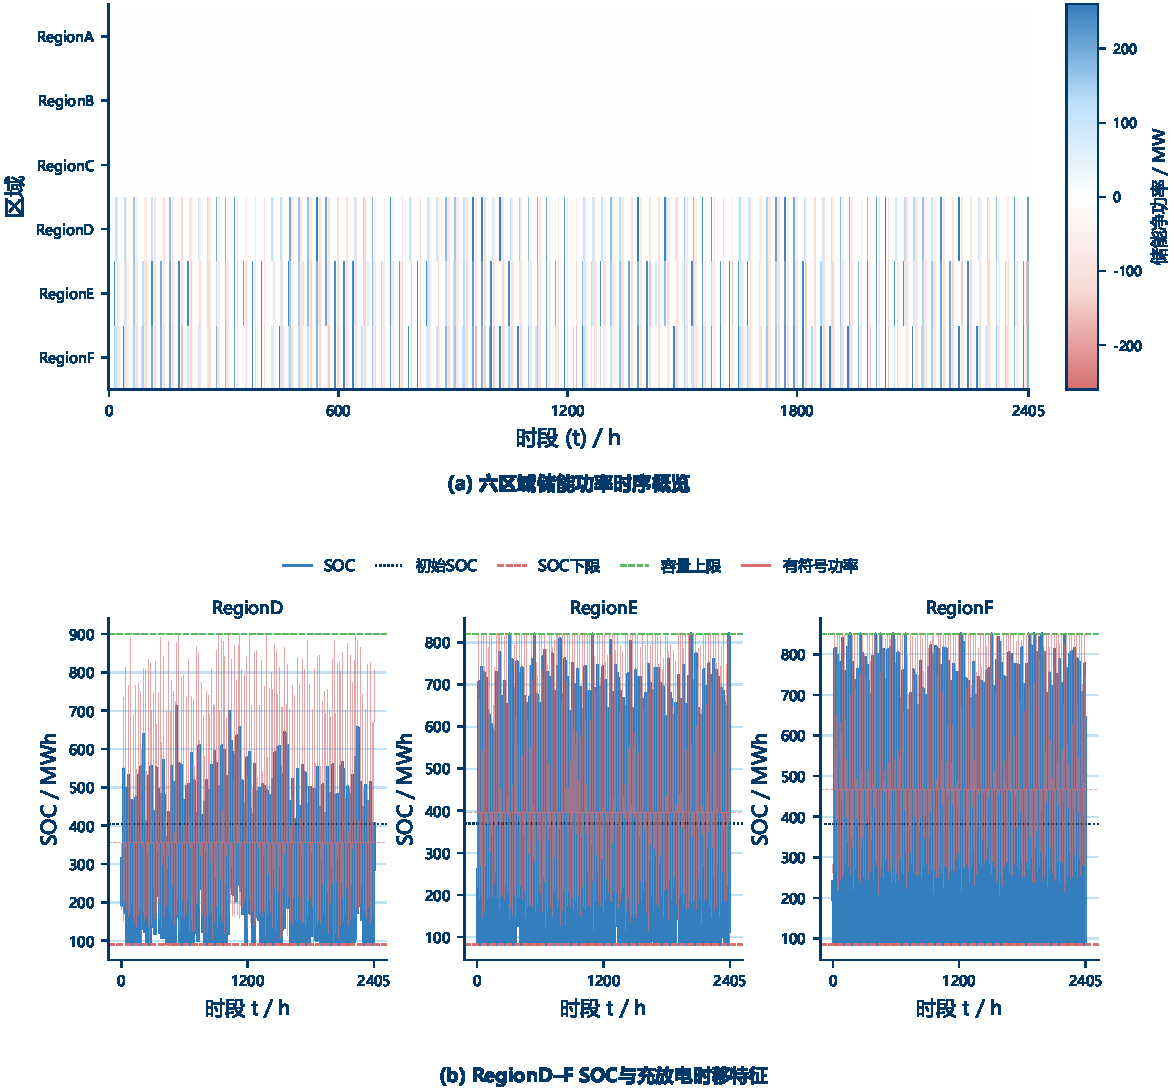
\includegraphics[width=0.92\textwidth]
	{figures/q3_group1_storage_mechanism.pdf}
    \caption{Storage power in six regions and SOC evolution in active regions}
	\label{fig:q3_storage}
\end{figure}

Storage is thus used mainly in regions with stronger regulation demand, rather than uniformly across regions.

The states supplied in the problem attachments are an operating reference only, not an optimization baseline in the same feasible set satisfying our terminal SOC condition. The no-storage schedule provides a model-consistent ablation.
The optimized operating cost is
$C=-4.5906\times10^{8}$,
with carbon emissions $E=0$,
the sum of six regional peak net purchases $P=0$,
and mean net purchase fluctuation $W=0.0113$ MW.
All four metrics improve on the attachment reference. Negative cost means export revenue exceeds purchase expenditure.

Zero emissions and peak net purchases do not imply zero data-center electricity load. Under the specified accounting rules, emissions arise only from grid purchases and the peak metric uses the positive part of net purchase power. For the present deterministic data and permitted renewable exports, renewables and storage supply the loads while surplus renewables are exported, reducing purchase-related emissions and positive net purchase peaks to zero. This depends on the current renewable, price, storage, and grid transaction conditions; zero values are not guaranteed under other parameter scenarios.

\begin{figure}[H]
	\centering
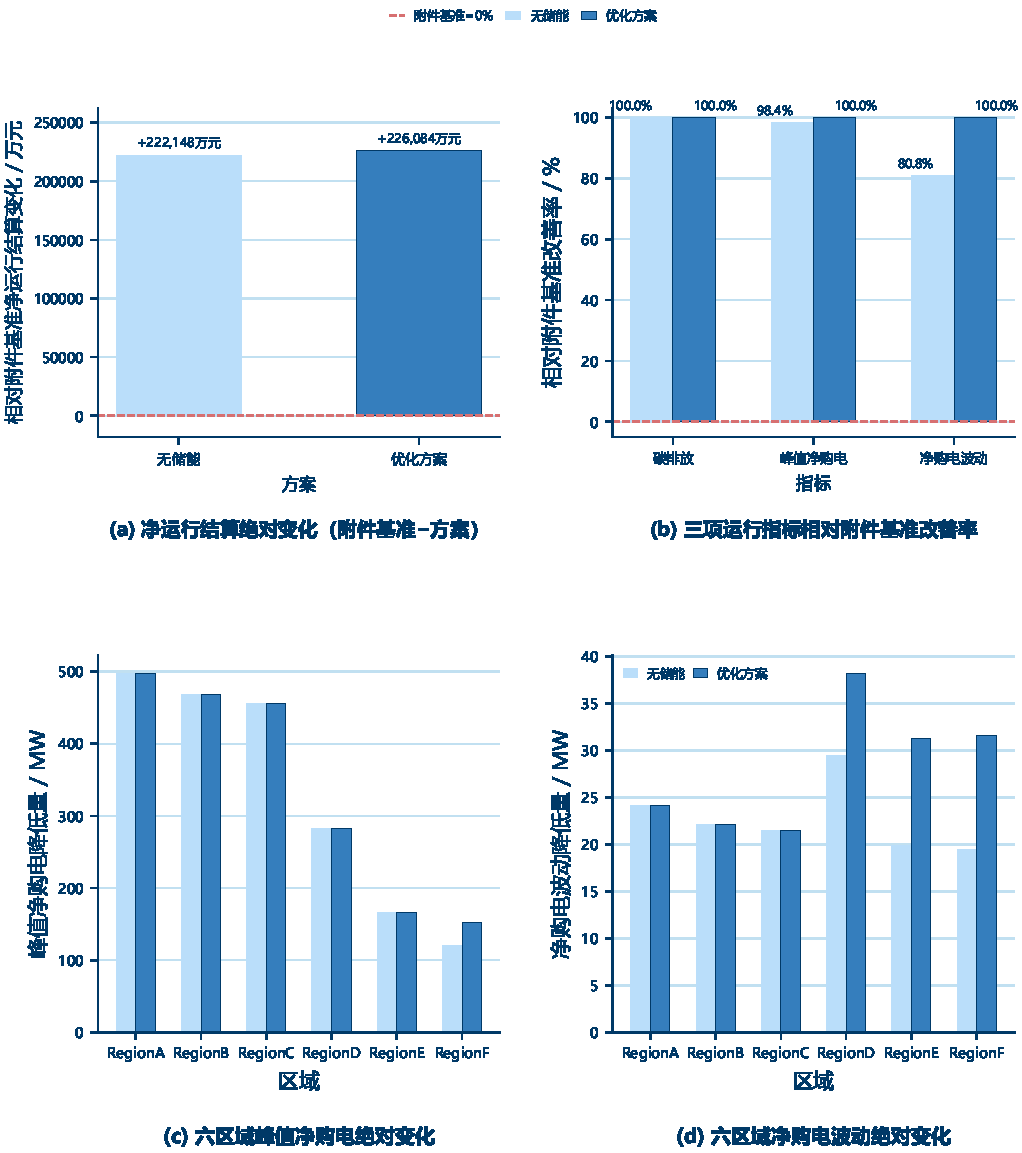
\includegraphics[width=0.86\textwidth]
{figures/q3_group2_optimization_effect.pdf}
\caption{Absolute net settlement changes, improvements in three metrics, and regional differences under storage coordination}
	\label{fig:q3_effect}
\end{figure}

Figure~\ref{fig:q3_effect} expresses absolute net settlement changes in CNY $10^4$ and the other metrics as relative improvements, avoiding ambiguous cost percentages when costs cross zero. All regional peaks fall; larger fluctuation improvements in RegionD--RegionF match the regions with active storage.

Set $C^{RE}_{rt}=C^G_{rt}=D_{rt}=0$ to construct a no-storage counterfactual.
Its operating cost is $-4.1969\times10^{8}$,
carbon emissions are $8.8506$,
peak net purchases are $31.5979$ MW,
and mean net purchase fluctuation is $5.3981$ MW.
Compared with this counterfactual, optimization reduces net operating cost by 3936.19 units of CNY $10^4$, as well as emissions, peaks, and fluctuations.

Independent verification confirms that both the optimized and no-storage schedules satisfy energy balance, SOC, capacity, exclusivity, grid transaction, and terminal constraints.
Maximum renewable and load balance residuals in the attachment operating reference are approximately
$2.0\times10^{-4}$ MW and $1.504\times10^{-4}$ MW,
consistent with the precision of the original data.
However, the maximum SOC recursion deviation is about $0.9999$ MWh,
and the terminal SOC deficit is approximately $193.3$ MWh.
The attachment states therefore serve as an operating reference, but are not a feasible optimization solution under our constraints.

\begin{figure}[H]
	\centering
	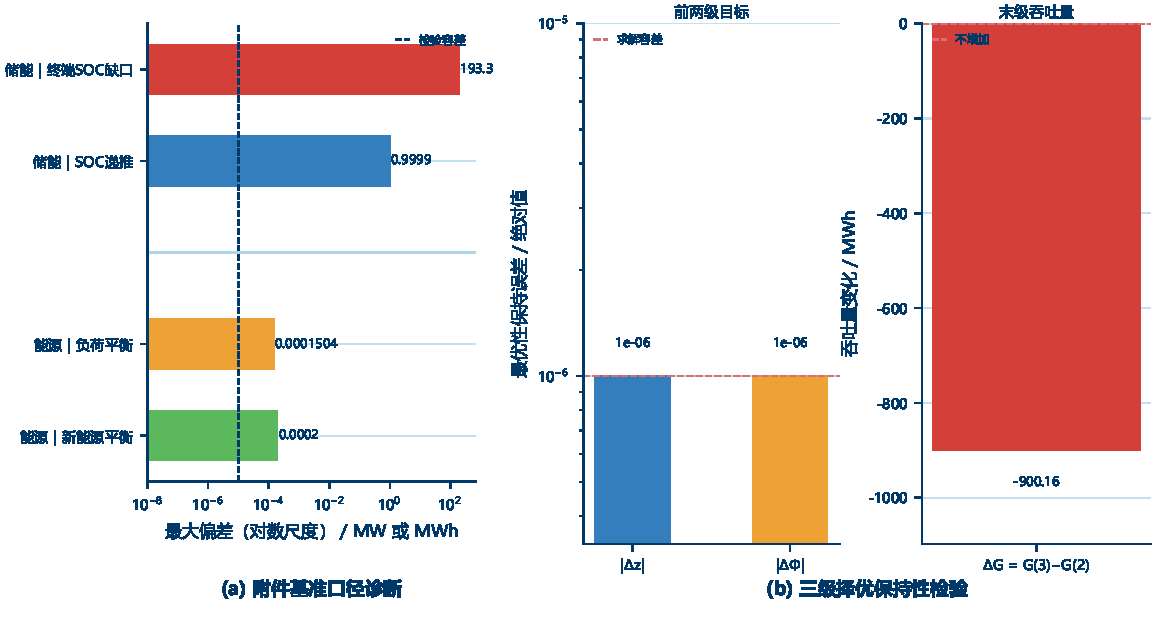
\includegraphics[width=0.91\textwidth]
	{figures/q3_group3_validation_credibility.pdf}
    \caption{Attachment-reference diagnostics and three-level multiobjective selection tests}
	\label{fig:q3_validation}
\end{figure}

In Figure~\ref{fig:q3_validation}, the third level changes $z$ and $\Phi$ by approximately $1.0\times10^{-6}$ relative to the preceding level while reducing storage throughput by 900.16 MWh. It reduces unnecessary cycling while retaining the first two levels' results.

Problem 3 quantifies intertemporal storage regulation under fixed loads and provides an energy-side baseline for Problem 4.



\section{Model Formulation and Solution for Problem 4}

\subsection{Model Formulation}

Problem 4 jointly optimizes job regions, start times, renewables, storage, and grid transactions. It initializes jobs with the feasible Problem 2 schedule and retains the energy mechanisms of Problem 3. Migration and time shifting affect renewable utilization, SOC, and grid exchanges through the PUE mapping, yielding a joint computing--storage--electricity model.

Spatial and temporal load shifting can coordinate with storage and electricity decisions\cite{ref9}. We retain deadlines, network latency, resource capacities, and energy limits, adding terminal SOC and rolling recoverability constraints.

The job-side feasible set follows Problem 1. Variables $x_{irs}$ and Equation~(\ref{eq:q1_overlap}) determine the AI IT load
$P_{rt}^{AI}=\sum_i\sum_{s\in S_i}p_i\rho_{ist}x_{irs}$,
and the facility load is
$F_{rt}=PUE_r(P_{rt}^{AI}+P_{rt}^{NonAI})$.
Each job executes exactly once. Real-time jobs start immediately; flexible jobs satisfy time windows, latency, GPU and power capacities, and the boundary at 2406.

The energy side retains Equations~(\ref{eq:q3_energy_balance}) and (\ref{eq:q3_soc}), their capacity, exclusivity, grid transaction, and export constraints, and $S_{r,2406}\geq S_{r0}$.

To prevent excessive early discharge in rolling optimization, an SOC recoverability condition is imposed at the end of each decision window:
\begin{equation}
	S_{r,\tau+H}
	\geq
	\max\left\{
	S_r^{\min},
	S_{r0}-
	\eta_r^cP_r^{ch,\max}(2406-\tau-H)
	\right\}.
	\label{eq:q4_soc_recovery}
\end{equation}

Equation~(\ref{eq:q4_soc_recovery}) preserves the theoretical ability to restore initial SOC within the remaining horizon and connects to the terminal constraint.

The six metrics are net operating settlement $C$, carbon emissions $E$, network latency $L$, waiting loss $J$, renewable nonutilization $Q$, and peak net purchases $P$. The first three follow Problems 2 and 3. Let $\underline{s}_i,\overline{s}_i$ denote valid start-time bounds for flexible jobs and $\omega_i$ latency-sensitive weights. Then
\begin{equation}
	\begin{aligned}
		J&=
		\frac{
			\displaystyle\sum_{i\in I^{\mathrm{flex}}_+}
			\omega_i
			\frac{s_i-\underline{s}_i}
			{\overline{s}_i-\underline{s}_i}}
		{\displaystyle\sum_{i\in I^{\mathrm{flex}}_+}\omega_i},
		\qquad QoS=1-J,\\
		Q&=
		\frac{\displaystyle\sum_r\sum_tR_{rt}}
		{\displaystyle\sum_r\sum_tP^{RE}_{rt}},
		\qquad U=1-Q,\\
		P&=\sum_rP_r^{\max},
		\qquad
		P_r^{\max}\geq B_{rt}-X_{rt},
		\quad P_r^{\max}\geq0.
	\end{aligned}
	\label{eq:q4_metrics}
\end{equation}

Global centers $a_m$ and scales $R_m$ are fixed before rolling optimization and remain unchanged across windows and scenarios. The nondegenerate active metric set is $\mathcal M_{\mathrm{act}}=\{L,J,Q\}$.
Normalized deviations and the augmented minimax criterion for window $\tau$ are
\begin{equation}
	\begin{aligned}
		d_{m,\tau}
		&=
		\max\left\{
		0,\,
		\frac{\hat f_{m,\tau}-a_m}{R_m}
		\right\},
		\qquad m\in\mathcal M_{\mathrm{act}},\\
		\min\quad Z_\tau
		&=
		z_\tau+\eta\sum_{m\in\mathcal M_{\mathrm{act}}} d_{m,\tau},
		\qquad
		d_{m,\tau}\leq z_\tau\quad(m\in\mathcal M_{\mathrm{act}}),
		\qquad
		\eta=10^{-3}.
	\end{aligned}
	\label{eq:q4_minmax}
\end{equation}

Equation~(\ref{eq:q4_minmax}) applies only to $\mathcal M_{\mathrm{act}}$. Metrics $C,E,P$ are independently recomputed for evaluation and scenario comparisons. All six form a common evaluation system, but they are not equally active optimization objectives.

The full-horizon joint integer model is too large. We use a rolling matheuristic initialized by the Problem 2 schedule, with $H=24$ h, $K=48$ h, and an internal advancement of 4 h. The look-ahead interval supplies future information only. Table~\ref{tab:q4_algorithm} summarizes the procedure.

\begin{table}[H]
	\centering
    \caption{Rolling joint computing--storage--electricity optimization for Problem 4}
	\label{tab:q4_algorithm}

	\fontsize{10.5pt}{12pt}\selectfont
	\renewcommand{\arraystretch}{0.88}

	\begin{tabular}{
			>{\centering\arraybackslash}p{0.08\textwidth}
			>{\raggedright\arraybackslash}p{0.86\textwidth}}
		\toprule
        \textbf{Step} & \multicolumn{1}{c}{\textbf{Operation}}\\
		\midrule

        1 & Read the Problem 2 seed schedule, current SOC, historical peaks, and remaining-job states.\\

        2 & Reoptimize storage and grid responses over the $H=24$ h decision window and $K=48$ h look-ahead interval.\\

        3 & Use marginal linear programs to assess the potential joint-objective effects of migrating or shifting flexible jobs.\\

        4 & Use small mixed-integer linear programs to repair local adjustments that create resource conflicts.\\

        5 & Form a large neighborhood of key jobs and jointly release job and energy variables for refinement.\\

        6 & Commit feasible decisions for the current $H$ hours; update SOC, historical peaks, cumulative emissions, and remaining jobs.\\

		\bottomrule
	\end{tabular}
\end{table}


The joint large neighborhood releases execution regions, start times, and energy variables together. It accepts only schedules satisfying every hard constraint and improving Equation~(\ref{eq:q4_minmax}). The result is a computationally efficient feasible schedule satisfying all hard constraints; global optimality is not claimed.

The sequential baseline fixes the Problem 2 job schedule and then optimizes storage and grid transactions using the Problem 3 energy model. Both schedules use the same six evaluation metrics.

Job, network, capacity, and storage parameters remain fixed while carbon constraints, pricing mechanisms, and renewable fluctuations vary. Let $E^0$ denote baseline emissions, $E^{LC}$ a low-carbon reference, and $\gamma$ a renewable smoothing parameter. The three scenario families are
\begin{equation}
	\begin{aligned}
		E
		&\leq
		E^0-\lambda(E^0-E^{LC}),
		\qquad 0\leq\lambda\leq1,\\
		\pi_{rt}^{fix}
		&=\bar{\pi}_r,
		\qquad
		\sigma_{rt}^{fix}=\bar{\sigma}_r,\\
		P_{rt}^{RE}(\gamma)
		&=
		(1-\gamma)P_{rt}^{RE}
		+\gamma\bar P_{rd}^{RE,+},
		\qquad
		t\in\mathcal H_{rd}^{+}.
	\end{aligned}
	\label{eq:q4_scenarios}
\end{equation}

Renewable smoothing applies only to originally nonzero periods and preserves daily total energy. All scenarios retain the fixed normalization scales.

Finally, the job table and complete SOC trajectories reconstruct profiles for hours 0--2405, allowing consistent recomputation of all six metrics and hard constraints.

\subsection{Results and Model Validation}

With $H=24$ h and $K=48$ h, 50000 jobs are processed through 101 rolling windows. Only decision-window results satisfying all hard constraints are committed, followed by full-horizon recomputation.

Degenerate reporting metrics in the earlier sequential energy solution produced a comparison baseline with limited physical meaning. To remove that effect, we fix both the Problem 2 sequential job schedule and the existing joint job schedule, then reoptimize storage and grid transactions using identical energy-response rules. This step consistently recomputes the two schedules' energy trajectories; it is not a rerun of the complete joint search. Table~\ref{tab:q4_result} gives the results.

\begin{table}[H]
	\centering
    \caption{Joint and sequential job schedules under consistent energy accounting}
	\label{tab:q4_result}

	\fontsize{10.5pt}{12pt}\selectfont
	\renewcommand{\arraystretch}{0.90}

	\begin{tabular}{lrr}
		\toprule
        \multicolumn{1}{c}{\textbf{Metric}}
        & \multicolumn{1}{c}{\textbf{Sequential jobs}}
        & \multicolumn{1}{c}{\textbf{Joint jobs}}\\
		\midrule

        Net settlement/CNY
		& $-4.532307\times10^8$
		& $-4.538873\times10^8$\\

        Emissions/tCO$_2$
		& 30.1233
		& 71.2005\\

        Mean network latency/ms
		& 12.9468
		& 9.9618\\

        QoS loss
		& 0.083659
		& 0.079281\\

        Renewable nonutilization
		& 29.8615\%
		& 29.8357\%\\

        Peak net purchases/MW
		& 66.5709
		& 97.1828\\

		\bottomrule
	\end{tabular}
\end{table}


In Table~\ref{tab:q4_result}, the joint job schedule lowers net settlement by $6.5665\times10^5$ CNY, latency by 2.9851 ms, QoS loss by 0.004378, and renewable nonutilization by 0.0258 percentage points. Emissions increase by 41.0772 tCO$_2$ and peak net purchases by 30.6119 MW. Negative settlement means export revenue exceeds purchase expenditure. Joint job adjustments mainly improve service quality and slightly reduce net settlement and curtailment; they do not improve all six metrics simultaneously.

The two schedules therefore cannot be ranked independently of decision preferences. A scheduler prioritizing latency, waiting loss, and renewable utilization while accepting increased emissions and peak purchases may choose the joint schedule. If emissions or peak purchases are strictly controlled, a schedule from the corresponding constrained scenario should be used. We interpret the results as feasible strategies for different operating preferences, rather than a unique optimum independent of application conditions.

\begin{figure}[H]
	\centering
	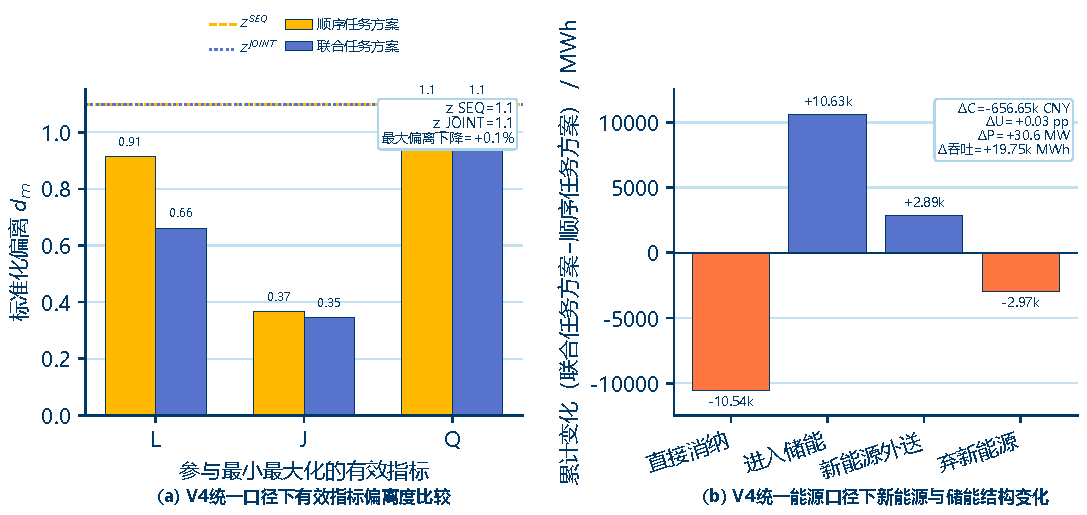
\includegraphics[width=0.88\textwidth]
	{figures/q4_group1_joint_optimization_results.pdf}
    \caption{Active metrics and renewable--storage structures of two job schedules under consistent energy accounting}
	\label{fig:q4_joint_result}
\end{figure}

In Figure~\ref{fig:q4_joint_result}, relative to sequential jobs, joint jobs reduce direct renewable use by $10.54\times10^3$ MWh, increase storage charging and exports by $10.63\times10^3$ and $2.89\times10^3$ MWh, reduce curtailment by $2.97\times10^3$ MWh, and increase storage throughput by $19.75\times10^3$ MWh. Metrics $L,J,Q$ are the nondegenerate active metrics actually used in the existing joint search. Metrics $C,E,P$ are independently recomputed with consistent energy accounting to report energy-side costs; they are not retrospectively described as joint-search objectives.

Equation~(\ref{eq:q4_scenarios}) defines carbon-constrained, fixed-price, and renewable-smoothing scenarios. Figure~\ref{fig:q4_scenario} shows changes relative to the joint baseline. It retains the completed scenario group and the joint baseline of that same version, comparing only within-group relative responses. Fixed-job energy recomputation in Table~\ref{tab:q4_result} and Figure~\ref{fig:q4_joint_result} specifically corrects the sequential--joint comparison. Absolute quantities from these two result groups are not combined.

\begin{figure}[H]
	\centering
	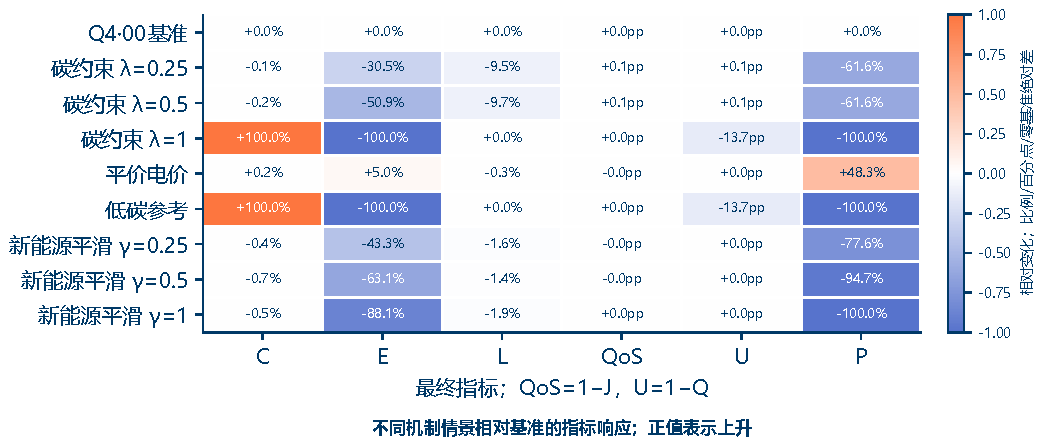
\includegraphics[width=0.86\textwidth]
	{figures/q4_group2_scenario_response.pdf}
    \caption{Scenario responses relative to the Problem 4 baseline}
	\label{fig:q4_scenario}
\end{figure}

In Figure~\ref{fig:q4_scenario}, increasing $\lambda$ from 0.25 to 0.50 lowers emissions from 297.36 to 209.97 tCO$_2$, with peaks around 95.54 MW and latency changing from 9.0144 to 8.9945 ms.
At $\lambda=1$, emissions and peak net purchases approach zero,
but renewable nonutilization rises to 43.5710\%.
Further restricting purchases therefore sacrifices renewable utilization rather than improving all metrics simultaneously.

Fixed electricity prices yield emissions of 449.37 tCO$_2$ and a peak of 368.71 MW. In renewable-smoothing scenarios,
for $\gamma=0.25,0.50,1.00$,
emissions are approximately 242.89, 158.01, and 50.85 tCO$_2$,
peak net purchases are approximately 55.73, 13.18, and 0 MW,
and latency remains within 9.77--9.81 ms. Smoothing mainly changes energy-side states.

Validation combines independent full-horizon recomputation with complete mixed-integer linear programs for representative windows. Both sequential and joint job schedules pass all 67 checks of jobs, capacity, latency, energy, SOC, and grid transactions. The largest hard-constraint violation is
$2.3842\times10^{-7}$, below the $10^{-6}$ verification tolerance.
The largest discrepancy between independently recomputed metrics and summary results is no greater than this order of magnitude.

\begin{figure}[H]
	\centering
	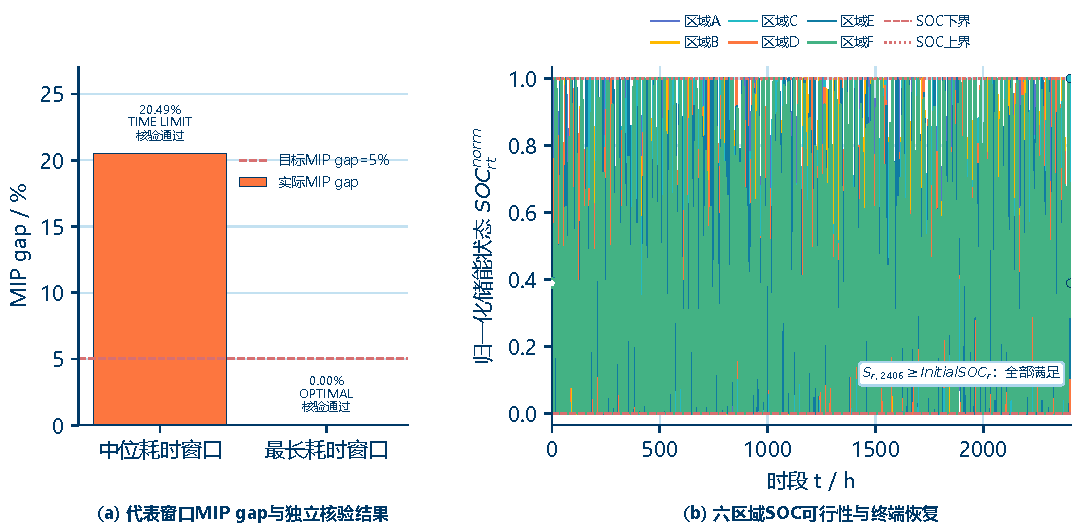
\includegraphics[width=0.88\textwidth]
	{figures/q4_group3_model_validation.pdf}
    \caption{Independent checks of complete representative-window mixed-integer models and six-region storage states}
	\label{fig:q4_validation}
\end{figure}

Figure~\ref{fig:q4_validation}(a) compares complete joint mixed-integer linear programs for windows 1512 and 2232. The former obtains a feasible reference with a 20.49\% relative gap within 600 s; the latter reaches optimality. Both pass constraint checks. This provides local feasibility and limited solution-quality references, not proof of full-horizon near-optimality or global optimality.

Figure~\ref{fig:q4_validation}(b) shows SOC trajectories for the joint job schedule after consistent energy recomputation. SOC stays within its bounds and satisfies $S_{r,2406}\geq S_{r0}$; benefits are not obtained by depleting initial stored energy.

Under the current data, the joint job schedule improves latency, waiting loss, and renewable nonutilization while increasing emissions and peak net purchases. Joint decisions therefore produce trade-offs rather than simultaneous superiority in all six metrics. Both schedules satisfy all job, computing, energy, and storage hard constraints. The conclusions concern computationally efficient feasible solutions; global optimality is not claimed, and fixed-job energy recomputation is not equated with complete joint search.

	\section{Model Evaluation and Extensions}

\subsection{Strengths}

\begin{enumerate}
    \item \textbf{Hierarchical forecasting preserves heterogeneity and consistency:}
    Problem 1 recovers 18 cross-classified demands from three forecast levels. Validation and test WAPE are 0.7241 and 0.6519, and all 84 rolling windows outperform the 24-hour same-hour baseline.
	
    \item \textbf{Multiobjective scheduling exposes practical trade-offs:}
    Problem 2 uses fixed normalization, and full-horizon recomputation confirms that all 50000 jobs satisfy hard constraints. Cost falls by 507.34 units of CNY $10^4$ and renewable utilization rises by 0.223 percentage points, with the increased emissions and latency also reported.
	
    \item \textbf{The storage model retains the specified load convention:}
    Problem 3 fixes the specified loads and optimizes only energy decisions. Relative to no storage, cost falls by 3936.19 units of CNY $10^4$, with lower emissions, peaks, and fluctuations. SOC and terminal constraints pass verification.
	
    \item \textbf{Joint scheduling captures computing--storage--electricity interactions:}
    Problem 4 recomputes sequential and joint job schedules with consistent energy accounting. Joint jobs lower cost by 65.67 units of CNY $10^4$, mean latency by 2.9851 ms, and renewable nonutilization by 0.0258 percentage points, while raising emissions and peaks by 41.08 tCO$_2$ and 30.61 MW. This fully reports the energy-side cost of service-quality improvements. Both schedules pass all 67 independent checks.
\end{enumerate}


\subsection{Limitations}

\begin{enumerate}
    \item \textbf{Forecasts depend on stable recent demand structure:}
    Recovery of the 18 demands relies on historical structure, and its accuracy change relative to direct forecasting is not statistically significant ($p=0.2163$). Abrupt business changes require dynamic windows or time-varying weights.
	
    \item \textbf{The Problem 2 rolling heuristic does not guarantee global optimality:}
    The maximum normalized-objective deviation from exact models in difficult windows is 293.40\%. Resource-constrained neighborhoods could be expanded and critical windows given longer solve times.
	
    \item \textbf{Extreme scenarios and uncertainty receive limited treatment:}
    Problems 3 and 4 use deterministic prices, carbon intensity, and renewable sequences, excluding forecasting errors and storage degradation. Progressively tightened constraints and robust or stochastic optimization could be introduced.
\end{enumerate}


\subsection{Extensions}

The framework can support multiregional data centers, computing networks, and campus source--load--storage scheduling, but must be recalibrated to actual job windows, networks, capacities, PUE, prices, carbon intensity, renewables, storage, and SLAs. Introducing preemption, interregional electricity exchange, or forecasting errors requires additional state and uncertainty constraints and renewed validation. The transferable element is the modeling framework, not the parameters or numerical results in this paper.

	
    \section*{AI Tool Use Declaration}
    The team used DeepSeek during the competition,
    primarily for language editing, code debugging, figure preparation, and LaTeX typesetting assistance.
    Details are provided in the appendix.
	
	
	\referencescn
	
	\newpage
	\section*{Appendix}

\subsection*{A. Software Environment and Reproduction}

Calculations use Python 3.12.13, with NumPy, pandas, Matplotlib, Seaborn, OpenPyXL, SciPy, and HiGHS for scientific computing, data processing, plotting, and optimization. The environment is managed by \texttt{uv}. Dependency constraints and locked versions are recorded in \texttt{pyproject.toml} and \texttt{uv.lock} in the supporting materials.

To reproduce results, first synchronize the environment, then execute the problem-level entry points in order from Problem 1 to Problem 4, working in the repository's \texttt{code/} directory. Preprocessing for Problems 2--4 depends on the shared processed layer generated by Problem 1. Run:

\begin{lstlisting}[language={},basicstyle=\ttfamily\small]
uv sync
uv run python question\question_01\main.py
uv run python question\question_02\main.py
uv run python question\question_03\main.py
uv run python question\question_04\main.py
\end{lstlisting}

Each entry point performs data processing, model solving, validation, and plotting in sequence. The supporting materials retain processed model inputs and generated result tables. To check published values, inspect result and independent-verification tables directly. To recompute from raw attachments, repeat preprocessing while preserving the original problem data.

\subsection*{B. Source Code and Supporting Materials}

Supporting materials include all source programs, environment configuration, processed model inputs, key result and validation tables for Problems 1--4, paper figures, and file checksum inventories. Result tables trace specific reported values; figures present results; independent-verification tables check job coverage, resource capacity, energy balance, storage states, and time boundaries.

Problem-specific evidence includes demand forecasting, baseline scheduling, and stress boundaries for Problem 1; multiobjective scheduling, baseline comparison, resource--energy recomputation, and sensitivity tests for Problem 2; storage optimization, regional metrics, baseline checks, and constraint tests for Problem 3; and joint computing--storage--electricity scheduling, scenarios, representative-window tests, and independent verification for Problem 4.

\subsection*{C. Limits on Result Interpretation}

Reported values come from the corresponding result tables, not estimates from figures. Passing hard-constraint checks establishes feasibility only for the given data, parameters, and boundaries. It does not establish global optimality or universal superiority across scenarios. Matheuristic results are reported with their actual solution method, comparison tests, and remaining limitations.

Hours 0--2399 form the main operating period; hours 2400--2405 complete already arrived jobs; hour 2406 is the terminal settlement boundary, not an ordinary execution hour. Costs including electricity sale revenue are net settlement values and do not imply negative actual electricity consumption.

\subsection*{D. AI Tool Use Details}

The team used DeepSeek during the competition for language editing, code debugging, figure preparation, and LaTeX typesetting assistance. AI was not used to determine core models, formulas, parameters, raw data, or final conclusions.

\subsubsection*{D.1 Tool and Dates of Use}

\begin{table}[H]
    \centering
    \small
    \renewcommand{\arraystretch}{1.05}
    \setlength{\tabcolsep}{3pt}
    \begin{tabularx}{0.96\textwidth}{>{\centering\arraybackslash}p{0.18\textwidth}>{\centering\arraybackslash}p{0.20\textwidth}>{\centering\arraybackslash}X>{\centering\arraybackslash}p{0.22\textwidth}}
        \toprule
        AI tool & Version/model & Developer & Dates of use \\
        \midrule
        DeepSeek & DeepSeek-v4-flash-0731 & DeepSeek & August 7--10, 2026 \\
        \bottomrule
    \end{tabularx}
\end{table}

The model version used was DeepSeek-v4-flash-0731.

\subsubsection*{D.2 Activities and Purposes}

DeepSeek assisted with language editing, debugging, figure preparation, final-draft compression, terminology consistency, citations, result-version checks, and LaTeX review. AI neither generated nor altered raw data and did not change the objectives, constraints, or parameters of the existing joint job search. Additional results were generated by actual local execution and independently recomputed.

\subsubsection*{D.3 Key Interaction Records}

\noindent\textbf{Record 1: DeepSeek language assistance, August 7--10, 2026}

The prompt requested review only of text written by the team, with local revision suggestions and no new models, formulas, data, or conclusions. AI identified long sentences, repetition, inconsistent terminology, and weak connections between text and figures. The team manually screened, checked, and rephrased suggestions.

\noindent\textbf{Record 2: Code debugging and figure assistance, August 9, 2026}

The prompt restricted review to syntax, indexing, data types, file reading, and plotting parameters in existing programs. It prohibited changes to raw data, objectives, constraints, model structure, parameters, and final conclusions. AI suggested variable checks, index corrections, data-type conversions, and figure-label improvements. The team adopted only suggestions reproducible locally without changing model meaning.

\noindent\textbf{Record 3: DeepSeek final-draft review, August 10, 2026}

The prompt required strict review of Problem 4 result accounting against a checklist, removal of mixed data versions across the sequential baseline, joint schedule, figures, and text, and consistent academic language, citations, and LaTeX formatting. AI assisted in adding entry points for consistent fixed-job energy recomputation and independent verification, and in revising plotting and paper sources. Every new metric was generated by actual execution on the team's computer; the team performed final checks and submission.

\subsubsection*{D.4 Adoption and Manual Revision}

The team checked all AI suggestions before adoption. Core methods, formulas, parameters, results, and conclusions were determined by the team, and final programs, data, figures, and conclusions were locally executed and verified. Complete DeepSeek records are contained in the corresponding use report in the supporting materials.

AI-assistance statements in the programs refer to the code checks and revisions involving DeepSeek. Assistance was limited to program review, result checking, figure preparation, and paper formatting; it did not rewrite the existing joint job-search model.

\subsection*{E. Source Inventory and Attachment Location}

All 24 Python source programs used for this problem were included in the source-code directory of the separately submitted support ZIP instead of being reprinted in the paper. That attachment also contains \texttt{pyproject.toml}, \texttt{uv.lock}, processed model inputs, key result and validation tables, paper figures, and a SHA-256 checksum inventory. Raw data supplied by the competition were not duplicated. The local readable copy is named \texttt{CCM2601033-support.zip}; the original competition package is retained in the frozen archive.

The source programs follow the relative directories for Problems 1--4 and comprise 24 \texttt{.py} files. Reproduction uses the commands in Appendix A in sequence. Paper and support attachments were submitted separately. The original attachment name followed the required problem-choice, entry-number, and attachment format, and its size was kept below 20 MB.


\end{document}
